\PassOptionsToPackage{unicode=true}{hyperref} % options for packages loaded elsewhere
\PassOptionsToPackage{hyphens}{url}
%
\documentclass[
]{article}
\usepackage{lmodern}
\usepackage{amssymb,amsmath}
\usepackage{ifxetex,ifluatex}
\ifnum 0\ifxetex 1\fi\ifluatex 1\fi=0 % if pdftex
  \usepackage[T1]{fontenc}
  \usepackage[utf8]{inputenc}
  \usepackage{textcomp} % provides euro and other symbols
\else % if luatex or xelatex
  \usepackage{unicode-math}
  \defaultfontfeatures{Scale=MatchLowercase}
  \defaultfontfeatures[\rmfamily]{Ligatures=TeX,Scale=1}
\fi
% use upquote if available, for straight quotes in verbatim environments
\IfFileExists{upquote.sty}{\usepackage{upquote}}{}
\IfFileExists{microtype.sty}{% use microtype if available
  \usepackage[]{microtype}
  \UseMicrotypeSet[protrusion]{basicmath} % disable protrusion for tt fonts
}{}
\makeatletter
\@ifundefined{KOMAClassName}{% if non-KOMA class
  \IfFileExists{parskip.sty}{%
    \usepackage{parskip}
  }{% else
    \setlength{\parindent}{0pt}
    \setlength{\parskip}{6pt plus 2pt minus 1pt}}
}{% if KOMA class
  \KOMAoptions{parskip=half}}
\makeatother
\usepackage{xcolor}
\IfFileExists{xurl.sty}{\usepackage{xurl}}{} % add URL line breaks if available
\IfFileExists{bookmark.sty}{\usepackage{bookmark}}{\usepackage{hyperref}}
\hypersetup{
  pdftitle={Tropical Cyclone Bibliography},
  pdfauthor={Matthew Hughes},
  pdfborder={0 0 0},
  breaklinks=true}
\urlstyle{same}  % don't use monospace font for urls
\usepackage[margin=1in]{geometry}
\usepackage{graphicx,grffile}
\makeatletter
\def\maxwidth{\ifdim\Gin@nat@width>\linewidth\linewidth\else\Gin@nat@width\fi}
\def\maxheight{\ifdim\Gin@nat@height>\textheight\textheight\else\Gin@nat@height\fi}
\makeatother
% Scale images if necessary, so that they will not overflow the page
% margins by default, and it is still possible to overwrite the defaults
% using explicit options in \includegraphics[width, height, ...]{}
\setkeys{Gin}{width=\maxwidth,height=\maxheight,keepaspectratio}
\setlength{\emergencystretch}{3em}  % prevent overfull lines
\providecommand{\tightlist}{%
  \setlength{\itemsep}{0pt}\setlength{\parskip}{0pt}}
\setcounter{secnumdepth}{-2}
% Redefines (sub)paragraphs to behave more like sections
\ifx\paragraph\undefined\else
  \let\oldparagraph\paragraph
  \renewcommand{\paragraph}[1]{\oldparagraph{#1}\mbox{}}
\fi
\ifx\subparagraph\undefined\else
  \let\oldsubparagraph\subparagraph
  \renewcommand{\subparagraph}[1]{\oldsubparagraph{#1}\mbox{}}
\fi

% set default figure placement to htbp
\makeatletter
\def\fps@figure{htbp}
\makeatother


\title{Tropical Cyclone Bibliography}
\author{Matthew Hughes}
\date{February 7, 2020}

\begin{document}
\maketitle

\hypertarget{spatial-levels}{%
\section{Spatial levels}\label{spatial-levels}}

\begin{itemize}
\tightlist
\item
  Point location (latitude / longitude or address) of each subject
  (e.g., household, individual)

  \begin{itemize}
  \tightlist
  \item
    (Bayleyegn et al. 2006)
  \end{itemize}
\item
  Fine spatial resolution, but not individual level (e.g., tree
  mortality in small areas measured by remote sensing)

  \begin{itemize}
  \tightlist
  \item
    (Bianchette et al. 2009)
  \end{itemize}
\item
  ZIP code

  \begin{itemize}
  \tightlist
  \item
    (Bevilacqua et al. 2020) {[}double-check{]}
  \item
    (Lane et al. 2013)
  \end{itemize}
\item
  County / parish

  \begin{itemize}
  \tightlist
  \item
    (Kinney et al. 2008)
  \item
    (S. C. Grabich et al. 2016) {[}double-check{]}
  \item
    (S. Grabich et al. 2016) {[}double-check{]}
  \end{itemize}
\item
  State

  \begin{itemize}
  \tightlist
  \item
    (Jaycox et al. 2010) {[}double-check{]}
  \end{itemize}
\item
  Country (e.g., Puerto Rico)

  \begin{itemize}
  \tightlist
  \item
    (Scaramutti et al. 2019) {[}double-check{]}
  \end{itemize}
\end{itemize}

\hypertarget{time-scales}{%
\section{Time scales}\label{time-scales}}

\emph{Either the specific time scale used, or the finest resolution that
would likely be helpful given the study's outcome data.}

\begin{itemize}
\tightlist
\item
  Day

  \begin{itemize}
  \tightlist
  \item
    (Bayleyegn et al. 2006)
  \item
    (Pugatch 2019)
  \end{itemize}
\item
  Between day and week

  \begin{itemize}
  \tightlist
  \item
    (Hagy, Lehrter, and Murrell 2006)
  \end{itemize}
\item
  Week (often pregnancy outcomes, where gestational week is a factor)

  \begin{itemize}
  \tightlist
  \item
    (Kinney et al. 2008)
  \item
    (S. C. Grabich et al. 2016) {[}double-check{]}
  \item
    (S. Grabich et al. 2016) {[}double-check{]}
  \end{itemize}
\item
  Cumulative measure across storm event

  \begin{itemize}
  \tightlist
  \item
    (Jaycox et al. 2010)
  \item
    (Scaramutti et al. 2019)
  \item
    (Bianchette et al. 2009)
  \end{itemize}
\end{itemize}

\hypertarget{kinney2008autism}{%
\section{(Kinney et al. 2008)}\label{kinney2008autism}}

This study tested a hypothesis that the risk of autistic disorder
increases in a dose-response manner relative to the intensity of
prenatal storm exposure, and that sensitive periods of gestation exist
where these exposures are more likely to increase the risk of autistic
disorder. The study was conducted in Louisiana parishes that had been
hit by the storm centers from 1980 to 1995.

\hypertarget{temporal-scale}{%
\subsection{Temporal Scale}\label{temporal-scale}}

\begin{itemize}
\tightlist
\item
  Severe storms between 1980 and 1995 were identified.
\item
  ``To investigate how timing of storm exposure affected prevalence, the
  normal 40-week term of gestation was divided into five equal periods,
  each period being 8 weeks (or two four week''months``). Although the
  use of shorter gestational periods would have been desirable, it would
  have yielded too few AD cases in each period to provide adequate
  statistical power. Moreover, data on individual gestation lengths were
  not available, so 40-week gestations were assumed when estimating
  gestational age during storms.'' (Kinney et al. 2008)
\end{itemize}

\hypertarget{spatial-scale}{%
\subsection{Spatial Scale:}\label{spatial-scale}}

\begin{itemize}
\tightlist
\item
  ``National Weather Service maps of storm tracks were used to identify
  the parishes that were hit by the centers of each storm, and thus were
  likely to have experienced the most intense effects of the storm''
  (Kinney et al. 2008)
\item
  Parishes hit by the center of the storms were assumed to have
  withstanded the most intense effects of the storm.
\item
  Storms that were considered severe were identified using data from the
  National Weather Service on all hurricanes, tropical storms and floods
  that included the storms' dates, tracks, and degrees of destruction.
\item
  Three levels of storm exposure were assessed: High, Intermediate, and
  Low/Control exposure to the storm. Each level was assessed based on
  whether the exposure included both, one, or none of the exposure
  factors (Storm intensity, and storm vulnerability).
\end{itemize}

\hypertarget{exposure}{%
\subsection{Exposure:}\label{exposure}}

\begin{itemize}
\tightlist
\item
  Severity of prenatal storm exposure assessed two ways: intensity of
  storm's impact on parish, and how vulnerable residents would be if
  storm hit their parish. (Intensity and Vulnerability).
\item
  Three levels of storm exposure were assessed: High, Intermediate, and
  Low/Control exposure to the storm. High exposure meant that both
  severity factors were present (both Intensity AND Vulnerability),
  Intermediate exposure meant only one of these factors was present
  (either Intensity OR Vulnerability), and Low/Control exposure meant
  that neither of the factors were present.
\item
  Using data from NCHS, 40 week gestations were assumed to estimate the
  gestional age of babies during the storm, so that the researchers
  could count backwards from the date of birth.
\end{itemize}

\hypertarget{resultsoutcomes}{%
\subsection{Results/Outcomes:}\label{resultsoutcomes}}

\begin{itemize}
\tightlist
\item
  AD (Autistic Disorder) had significantly higher prevalence in those
  with higher prenatal storm exposure. AD Prevalence also depended on
  Prenatal Period of Storm Exposure (what gestational period the baby
  was in when the storm exposure occured)
\end{itemize}

\hypertarget{bayleyegn2006rapid}{%
\section{(Bayleyegn et al. 2006)}\label{bayleyegn2006rapid}}

This study was a rapid needs assessment conducted in Santa Rosa and
Escambia counties in the Florida Panhandle shortly after Hurricane Ivan
in September 2004. It was done using a survey, with the goal of seeing
what critical needs residents had following the storm, in terms of
utilities.

\hypertarget{temporal-scale-1}{%
\subsection{Temporal scale}\label{temporal-scale-1}}

\begin{itemize}
\tightlist
\item
  Survey instruments administered over 3 days, 6 days after Hurricane
  Ivan made landfall. Since they measured this in days, they probably
  were looking at the specific day that the storm passed as the ``day
  0'', and then looking at needs at specific day-level time points from
  that initial day, so they would need a daily temporal scale for other
  exposure data.
\end{itemize}

\hypertarget{spatial-scale-1}{%
\subsection{Spatial Scale:}\label{spatial-scale-1}}

\begin{itemize}
\tightlist
\item
  Escambia and Santa Rosa counties were identified as those most
  impacted by Hurricane Ivan by Florida Department of Health.
  \#\#\#{[}Was this based on a qualitative assessment, or on any type of
  measurements? If the latter, let's include any quantitative
  measurements they used here.{]}\#\#\# Probability Proportional to Size
  Sampling (modified from the WHO), was used to obtain a sample of 30
  clusters within these counties, which were put on maps given to
  interview teams.
\item
  7 households interviewed per cluster, for a total of 420 households
  interviewed.
\item
  Interviews administered asking for demographic info, housing info,
  damage info, etc.
\end{itemize}

\hypertarget{exposure-1}{%
\subsection{Exposure}\label{exposure-1}}

\begin{itemize}
\tightlist
\item
  Hurricane Ivan making landfall on the Florida panhandle was the
  exposure. The Florida Department of Public Health then made a
  determination of several of the hardest hit areas to study (and also
  the determination that the storm was severe enough to consider parts
  of Florida as exposed to a severe event and so in need of assessment
  for current needs). \#\#\#{[}No further analysis was used to quantify
  the intensity of exposure in the study areas?{]}\#\#\#
\end{itemize}

\hypertarget{resultsoutcomes-1}{%
\subsection{Results/Outcomes}\label{resultsoutcomes-1}}

\begin{itemize}
\tightlist
\item
  Most commonly reported ``Greatest needs'' were garbage pickup and
  restoration of electricity, after that it was access to medical care,
  medications, home repair, and ice.
\item
  Interviews and surveys were intended to look at what the health and
  safety impacts were after the hurricane, it turned out to be a wide
  variety of factors including poor environmental hygiene, living in
  damaged homes, sleep disturbance, respiratory problems, and the
  aformentioned ``Greatest Needs.''
\end{itemize}

\hypertarget{hagy2006effects}{%
\section{(Hagy, Lehrter, and Murrell 2006)}\label{hagy2006effects}}

This study investigated the evolution of water quality in Pensacola Bay
in Florida following Hurricane Ivan in 2004. The studies were conducted
monthly for several years following the storm.

\hypertarget{temporal-scale-2}{%
\subsection{Temporal Scale:}\label{temporal-scale-2}}

\begin{itemize}
\tightlist
\item
  Water quality surveys conducted monthly from 2000 to 2004, the final
  of these 48 surveys before the storm happened 15 days before it made
  landfall. Post Hurricane Ivan surveys were taken October 6 and
  November 5, or 20 and 50 days after the storm, and compared to the
  survey taken 15 days before the hurricane made landfall. The paper
  didn't mention anything about when or if the water quality tests went
  back to a monthly schedule, but teh 20 and 50 day surveys seemed to be
  intended entirely for assessing the hurricane's impact. \#\#\#{[}Could
  you clarify? Is it that there was this tighter schedule right after
  the storm, and then it moved to a monthly schedule for the following
  few years?{]}\#\#\#
\end{itemize}

\hypertarget{spatial-scale-2}{%
\subsection{Spatial Scale:}\label{spatial-scale-2}}

\begin{itemize}
\tightlist
\item
  Water quality surveys conducted at up to 15 sites located on two
  transects within the Pensacola Bay system. These sample site shad
  recorded Latitude and Longitudinal coordinates.
\end{itemize}

\begin{figure}

{\centering 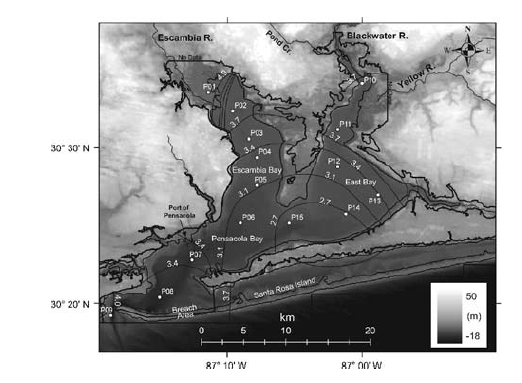
\includegraphics[width=0.4\textwidth]{figures/pensacola_bay_survey_sites} 

}

\caption{Example of how exposure to tornadoes was assesses in Christopher (2017) for counties.}\label{fig:unnamed-chunk-1}
\end{figure}

\begin{itemize}
\tightlist
\item
  The water quality surveys were really a series of tests described in
  the quotes: ``Hydrographic data were collected at each stationusing a
  Seabird SBE25 CTD measuring water temperature, salinity, dissolved
  oxygen, PAR, chlorophyll a fluorescence, and turbidity. Profile data
  were binned at a 0.25-m interval. Surface and bottom water samples
  were collected with either a Van Dorn bottle or a low pressure
  submersible pump. Samples for dissolved nutrients were filtered in the
  field using a syringe filter system with combusted GF/F filters.
  Additional 2-l water samples were collected in a clean polyethylene
  bottle and processed for chlorophyll a and particulate carbon and
  nitrogen in the laboratory within 2 to 3 h.'' (Hagy, Lehrter, and
  Murrell 2006)
\item
  If sample sites are given with lat./long., having point-level exposure
  data could help inform a study like this. Otherwise, watershed-level
  data (as well as, perhaps, data on a spatial scale linked to the water
  system, like ``bay'', ``inlet'', ``river'') might be more helpful.
\item
  ``River flow data were obtained from U.S. Geological Survey gauging
  stations on the Escambia River at Molino, Florida, Blackwater River
  near Baker, Florida, Yellow River near Milligan, Florida, and Big
  Coldwater Creek near Milton, Florida, accounting for 74\% of the
  watershed area. Runoff from ungauged watershed areas adjacent to
  Pensacola Bay was computed from the discharge per unit of watershed
  area in the Pond Creek watershed, a small gauged watershed immediately
  adjacent to Pensacola Bay'' (Hagy, Lehrter, and Murrell 2006)
\item
  The location and heights of high water marks around the perimeter of
  Pensacola Bay were used to estimate the extent of inundated land and
  the maximum height of the tidal surge.
\end{itemize}

\hypertarget{exposure-2}{%
\subsection{Exposure:}\label{exposure-2}}

\begin{itemize}
\tightlist
\item
  Exposure of interest in this study was the storm surge from Hurricane
  Ivan when it made landfall
\item
  Extent of inundated land and maximum height of tidal surge were
  estimated by directly observing locations and heights of high water
  marks around perimeter of Pensacola Bay.
\item
  Total Prism Model used to estimate the magnitude of exchange
  associated with storm surge.
\end{itemize}

\hypertarget{outcomeresults}{%
\subsection{Outcome/Results:}\label{outcomeresults}}

\begin{itemize}
\tightlist
\item
  Hurricane Ivan caused water to rise continuously for 31 hours.
\item
  Storm surge inundated 165 \(km^2\) of land, which increased the Bay's
  surface area by 50\% and it's volume by 230\%.
\item
  Based on Total Prism Model, storm surge flushed a maximum of 60\% of
  the Bay's water out to sea as it retreated---this must have increased
  salinity of the Bay substantially.
\item
  Using Navy's model estimate of offshore salinity in the Tidal Prism
  Model, Ivan's surge was computed to have increased the mean salinity
  of the Bay from 23.4 to as high as 30.0.
\item
  Tidal surge replaced Bay waters with low-nutrient, well-oxygenated,
  oligotrophic Gulf waters
\item
  Post-storm freshwater input stimulated an increase in phytoplankton
  biomass, which persisted for several weeks.
\item
  Hypoxia was intensified relative to the seasonal norm.
\end{itemize}

\hypertarget{lieberman2017self}{%
\section{(Lieberman-Cribbin et al. 2017)}\label{lieberman2017self}}

This study investigated how exposure to flooding during Hurricane Sandy
in 2012 was associated with mental health in New York City and Long
Island, NY. Self reported flooding exposure was compared to flooding
exposure data from FEMA after Hurricane Sandy and this then an
association was determined between the flooding exposure and depression,
anxiety, and PTSD.

\hypertarget{temporal-scale-3}{%
\subsection{Temporal Scale}\label{temporal-scale-3}}

\begin{itemize}
\tightlist
\item
  Surveys were all administered after Hurricane Sandy, and the mean time
  elapsed since Hurricane Sandy was 20.16 months.
\end{itemize}

\hypertarget{spatial-scale-3}{%
\subsection{Spatial Scale:}\label{spatial-scale-3}}

\begin{itemize}
\tightlist
\item
  A residential address for each study subject was then geocoded to a
  latitude and longitude (point location) for each study subject.
\item
  Street level geo-coding in SAS using datasets generated from U.S.
  Census Bureau TIGER/Line shapefiles. Process matches street, city, and
  zip-code from survey dataset with lookup dataset to produce a
  coordinate
\item
  Point-level, it sounds like (or at least street level)
\item
  ``In conjunction with community and governmental partners, the
  recruitment team traveled to libraries, community centers, senior
  centers, gyms and faith-based institutions across Queens, Staten
  Island, Nassau, and Suffolk in both heavily and less affected areas,
  and accepted all the volunteers who offered to participate in the
  study.'' (Lieberman-Cribbin et al. 2017)
\end{itemize}

\hypertarget{exposure-3}{%
\subsection{Exposure:}\label{exposure-3}}

\begin{itemize}
\tightlist
\item
  Extent of flooding at the study subject's residential address as a
  result of Hurricane Sandy in 2012
\item
  Flooding was the main factor for assessing hurricane exposure
\item
  FEMA dichotomous and FEMA continuous flooding models were used to map
  the flooding exposure in New York City and Long Island
\item
  Self-reported flooding exposure was also assessed and compared to the
  FEMA models. There were discrepencies between the two of these.
\item
  ``Public macro-level flood data was obtained from the FEMA Modeling
  Task Force (MOTF) Hurricane Sandy Impact Analysis'' (Lieberman-Cribbin
  et al. 2017)
\item
  New York State 3-meter spatial resolution storm surge product
  downloaded and imported into licensed version of ArcGIS to provide
  water depth above ground in New York City and Long Island
\item
  They also assessed the degree of exposure based on self reports of
  flooding water height.
\item
  Participants who did not provide an address were excluded from the
  study.
\item
  ``The presence and height of flooding were gathered from the overall
  hurricane exposure measure. Instances where participants recorded that
  there was no flooding in their home during Sandy (n = 63) were
  correspondingly assigned a flood height of 0 feet in order to be
  incorporated in a continuous measure of flood exposure. Instances
  where participants recorded flooding in their homes but did not record
  a numerical water height (n = 66) could not be included in analyses
  involving the continuous measure of flood exposure. A maximum water
  height of 15 feet reported on questionnaires was chosen as a cutoff to
  be included in this study to remove unreasonable flood heights. This
  choice excluded 4 participants.'' (Lieberman-Cribbin et al. 2017)
\item
  Self-reported flood data was collected, meaning that the subjects were
  asked to assess their own flood exposure. The address they provided
  was used to create a a point location using latitude and longitude
\item
  It sounds like they ideally wanted to match exposure to a point
  location (subject's home). They used a very fine-scale (3-m
  resolution) estimate of storm surge to try to do this (as well as
  asking the subject to assess their own flood exposure).
\end{itemize}

\hypertarget{resultsoutcomes-2}{%
\subsection{Results/Outcomes:}\label{resultsoutcomes-2}}

\begin{itemize}
\tightlist
\item
  Mental health variables considered based on scores of a questionaire
  were anxiety score, depression score, and PTSD score
\item
  Self reported flood exposure and FEMA flood exposure data showed
  significant discrepencies in the associations between flooding and
  mental health outcomes.
\item
  Self reported dichotomous flooding showed significant associations
  with all mental health outcomes, whereas dichotomous FEMA flooding
  only showed significant associations with PTSD.
\item
  Macro-level flooding data is less expensive and faster, but
  potentially underestimates mental health outcomes.
\end{itemize}

\hypertarget{grabich2016hurricane}{%
\section{(S. C. Grabich et al. 2016)}\label{grabich2016hurricane}}

This study investigated the association between risk of pre-term birth
and hurricane exposure in Florida.

\hypertarget{spatial-scale-4}{%
\subsection{Spatial Scale:}\label{spatial-scale-4}}

\begin{itemize}
\tightlist
\item
  Births to (only) Florida residents linked to address to link to
  hurricane exposure
\item
  Hurricane risk assessed at county level
\item
  Florida Department of Health, Vital Statistics Department was the
  source of data on births from 2003 to 2005.
\end{itemize}

\hypertarget{temporal-scale-4}{%
\subsection{Temporal Scale:}\label{temporal-scale-4}}

\begin{itemize}
\tightlist
\item
  Risk period begins at 20 weeks of gestation
\item
  Pregnancy divided into exposed time and unexposed time after 20 weeks
\item
  Study population included births with estimated date of conception
  between October 24, 2003 and September 26, 2004.
\item
  ``The authors used county-level Vital Statistics data obtained from
  the Florida Department of Health to calculate county-specific rates
  oflow birth weight and preterm births for women who were pregnant
  during the 2004 hurricane season. Women included in this calculation
  had an estimated date of conception based on last menstrual period
  between October 2003 and September 2004. These women would be at risk
  of hurricane exposure during pregnancy.'' (S. C. Grabich et al. 2016)
\end{itemize}

\hypertarget{exposure-4}{%
\subsection{Exposure:}\label{exposure-4}}

\begin{itemize}
\tightlist
\item
  Hurricane exposure classified as maximum wind speed in specific
  Florida county extracted from NOAA's Hurricane Research Division
  public database.
\item
  ``Wind speeds were extracted from NOAA's Hurricane Research Division
  (HRD) public databases.'' (S. C. Grabich et al. 2016)
\item
  ``The geographic spatial buffer exposure method yielded different
  results than either the disaster declaration method or the binary
  maximum wind-speed-exposure classifications. For all hurricanes except
  Hurricane Ivan, the 60 and 100-km buffer identified a similar number
  of counties as the binary 63-km=h (39-mi=h) windspeed categorization.
  For Hurricane Ivan, the number of counties exposed to both the 60 and
  100-km buffer was less than any of the other methods. Compared with
  the counties exposed using the dichotomous 119-km=h (74-mi=h) maximum
  wind speed, there was a 138\% difference in the number of counties
  exposed. Although the spatial buffer categorized a similar number of
  counties exposed as the binary wind speed methods, the heterogeneity
  across storms is apparent, particularly for Hurricane Ivan.''(S. C.
  Grabich et al. 2016)
\end{itemize}

\#\#\#{[}Could you check on this---did they use the wind field value for
the county, for example from H*Winds, or did they use the central wind
of the storm as the approximation, which they would have gotten from
HURDAT?{]}\#\#\# - Exposure defined as \textgreater{}= 39 mph and
\textgreater{}= 74 mph

\hypertarget{resultsoutcomes-3}{%
\section{Results/Outcomes}\label{resultsoutcomes-3}}

\begin{itemize}
\tightlist
\item
  Outcome of interest was to see if there was an association between
  hurricane exposure and the risk of a preterm birth.
\item
  Two outcome standards: extremely preterm delivery \textless{} 32 weeks
  gestation, and overall preterm delivery \textless{} 37 weeks
  gestation.
\item
  Overall positive association observed between exposure to Hurricane
  Harvey and hazard of extreme preterm delivery (not overall preterm
  delivery however)
\end{itemize}

\hypertarget{scaramutti2019mental}{%
\section{(Scaramutti et al. 2019)}\label{scaramutti2019mental}}

This study investigated mental health outcomes in Puerto Ricans in both
Puerto Rico and Florida following Hurricane Maria through a survey-based
study.

\hypertarget{spatial-scale-5}{%
\subsection{Spatial Scale:}\label{spatial-scale-5}}

\begin{itemize}
\tightlist
\item
  Major cities in Florida and Puerto Rico were coded as urban with 0,
  and all other areas were coded as rural/suburban with a 1.
\item
  Word of mouth and outreach to community leaders and community centers
  in Central and South Florida and Puerto Rico
\item
  Online surveys available through Qualtrics, respondants asked to refer
  3 additional respondants
\item
  \#\#\#{[}Do we know if they had the exact address of each participant?
  Or did they only know that they were in Puerto Rico and whether they
  were in the city or a rural area, without knowing which city or
  area?{]}\#\#\# It doesn't appear that the exact address of the
  respondants was provided, and seems unlikely given that the identities
  of the participants were not even verifiable.
\end{itemize}

\hypertarget{temporal-scale-5}{%
\subsection{Temporal Scale:}\label{temporal-scale-5}}

\begin{itemize}
\tightlist
\item
  Assessing mental health of Puerto Ricans in Florida and Puerto Rico 6
  months after Hurricane Maria.
\item
  There was a single time point when outcomes were measured, so coarser
  time resolutions (e.g., week, month, single value for the storm as a
  whole) would probably be useful in this type of study.
\end{itemize}

\hypertarget{resultsoutcomes-4}{%
\subsection{Results/Outcomes:}\label{resultsoutcomes-4}}

\begin{itemize}
\tightlist
\item
  Linear regression models used with site and urbanacity as predictors
  for depressive symptoms, anxiety symptoms, and PTSD symptoms
\item
  Binary logistic regression analysis for clinical vs non-clinical
  anxiety, depression, and PTSD as criterion variables, and site or
  urbanacity as predictors
\item
  Mental health outcomes of interest were anxiety, depression, and PTSD
\item
  Results showed significant associations between urbanacity and
  anxiety, approaching statistical significance for association between
  urbanacity and depressive symptoms, and significant association
  between urbanacity and PTSD intrusive reexperiencing and PTSD
  hypervigilance.
\item
  Overall, rates of depression and PTSD were higher in Puerto Ricans who
  migrated to Florida after Hurricane Maria.
\item
  Puerto Ricans outside major cities were more likely to meet criteria
  for depression and PTSD
\item
  Puerto Ricans in Puerto Rico had significantly fewere clinical
  symptoms than those in Florida, but rates were high overall for both
  Florida and Puerto Rico.
\end{itemize}

\hypertarget{bianchette2009ecological}{%
\section{(Bianchette et al. 2009)}\label{bianchette2009ecological}}

This study investigated the ecological impacts (particularly in terms of
tree mortality) in a coastal area in Alabama following Hurricane Ivan in
2004.

\hypertarget{temporal-scale-6}{%
\subsection{Temporal Scale:}\label{temporal-scale-6}}

\begin{itemize}
\tightlist
\item
  Post hurricane images of vegetation take 9.5 months after hurricane to
  ensure that vegetation damage observed was permanent.
\end{itemize}

\hypertarget{spatial-scale-6}{%
\subsection{Spatial Scale:}\label{spatial-scale-6}}

\begin{itemize}
\tightlist
\item
  Study area was three coastal lakes known as the Shelby Lakes in Gulf
  State Park, Alabama.
\item
  Remote sensing using Landsat 5 images coupled with ground surveys of
  tree mortality were used.
\item
  ``Two Landsat 5 images (30 m resolution, path 020, row 039, GeoTiff
  format), dated 20 July 2004 (pre-Ivan) and 7 July 2005 (post-Ivan),
  were used for this study.'' (Bianchette et al. 2009)
\end{itemize}

\hypertarget{exposure-5}{%
\subsection{Exposure:}\label{exposure-5}}

\begin{itemize}
\tightlist
\item
  Hurricane Ivan brought 120 mph winds and a storm surge of 10-12 feet,
  which inundated all of the coastal plane around the Shelby Lakes.
\item
  \#\#\#It sounds like the full study area was assumed to be exposed
  based on the fact that the whole area around it was inundated by the
  surge of this storm?\#\#\#
\end{itemize}

\hypertarget{resultsoutcomes-5}{%
\subsection{Results/Outcomes:}\label{resultsoutcomes-5}}

\begin{itemize}
\tightlist
\item
  Ecological impacts were the main concern of this study, primarily
  measured by tree mortality.
\item
  Trees at lower elevation showed greater mortality than those at higher
  elevations.
\item
  Results suggested that saltwater intrusion and storm surge flooding
  were the main reasons for tree mortality in forests around Shelby
  Lakes, rather than wind damage.
\end{itemize}

\hypertarget{grabich2016measuring}{%
\section{(S. Grabich et al. 2016)}\label{grabich2016measuring}}

This study investigated the association between hurricane exposure and
birth outcomes in Florida. In particular, it investigated different ways
of assessing exposure to the storm. At the time of publishing, the most
accepted methods for assigning disaster exposure: FEMA presidential
disaster declarations and spatial data on the specific storm track
trajectory. The authors of this paper propose a new method that uses
meteorological data to define exposure to hurricanes.

\hypertarget{spatial-scale-7}{%
\subsection{Spatial Scale:}\label{spatial-scale-7}}

\begin{itemize}
\tightlist
\item
  Preterm birth and low birth weight rates collected from the county
  level of exposed areas
\item
  ``The authors' novel meteorological method uses the hurricane
  intensity by the county's maximum wind speed. Wind speeds were
  extracted from NOAA's Hurricane Research Division (HRD) public
  databases.'' (S. Grabich et al. 2016)
\end{itemize}

\hypertarget{temporal-scale-7}{%
\subsection{Temporal Scale:}\label{temporal-scale-7}}

\begin{itemize}
\tightlist
\item
  In other birth outcome studies, it seems like gestational week might
  be used a lot? So, this study might not need a higher resolution than
  week? It's interesting, since they have three different exposure
  metrics, they really have two different time resolutions on those. The
  winds and storm track could be determined to about the hour (and
  certainly the day), while the FEMA disaster declarations will be a
  single, storm-long measurement (the storm resulted in one or it
  didn't).
\end{itemize}

\hypertarget{exposure-6}{%
\subsection{Exposure:}\label{exposure-6}}

\begin{itemize}
\tightlist
\item
  Hurricane disaster exposure 3 methods, FEMA Presidential disaster
  declarations, spatial data on specific storm trajectory (storm tracks
  with a symmmetrical buffer around them), novel meteorological measure
  based on Saffir-Simpson hurricane intensity scale {[}i.e., including
  wind speeds experienced locally{]}. \textbackslash{}begin\{figure\}
\end{itemize}

\{\centering 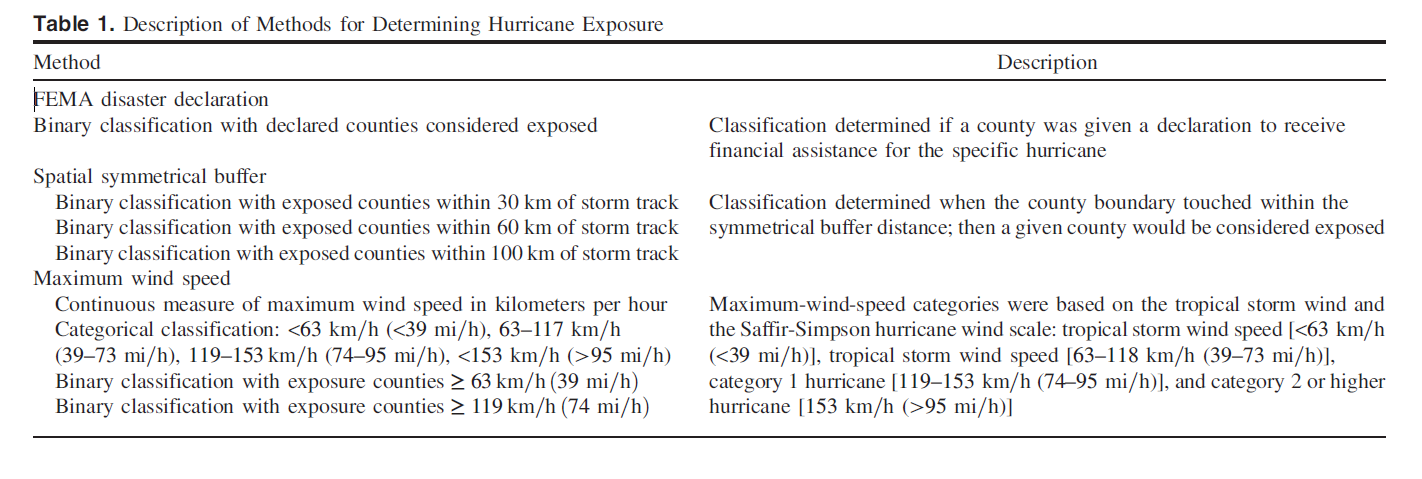
\includegraphics[width=0.4\textwidth]{figures/grabich_hurricane_exposure_methods}

\}

\caption{Example of how exposure to tornadoes was assesses in Christopher (2017) for counties.}\label{fig:unnamed-chunk-2}

\textbackslash{}end\{figure\}

\hypertarget{resultsoutcomes-6}{%
\subsection{Results/Outcomes:}\label{resultsoutcomes-6}}

\begin{itemize}
\tightlist
\item
  All three of the different exposure methods showed noticeably
  different results. The FEMA disaster declaration consistently assigned
  the highest number of counties as exposed, and the authors speculate
  that it could be overassigning.
\item
  Using the disaster declaration method, the authors could not find any
  statistically significant associations between the whether the county
  was exposed, and low-birth weight and pre-term births, but these null
  findings support the idea that exposure misclassification is
  occurring.
\end{itemize}

\hypertarget{bevilacqua2020understanding}{%
\section{(Bevilacqua et al. 2020)}\label{bevilacqua2020understanding}}

This study investigated associations between exposure to Hurricane
Harvey in 2017, and mental health symptoms in the Greater Houston Area.

\hypertarget{spatial-scale-8}{%
\subsection{Spatial Scale:}\label{spatial-scale-8}}

\begin{itemize}
\tightlist
\item
  The Greater Houston Area was the study area and spatial scale of this
  study. Recruitment events were organized in different neighborhooods
  of Houston to get participants to enroll.
\item
  Efforts were made to recruit a sample of participants that reflected
  the racial/ethnic makeup of Houston.
\item
  ggmaps package in R was used to generate distribution of zip codes of
  the participants
\end{itemize}

\hypertarget{temporal-scale-8}{%
\subsection{Temporal Scale:}\label{temporal-scale-8}}

\begin{itemize}
\tightlist
\item
  Study began 5 months post-Hurricane Harvey in January of 2018, and
  survey participants were recruited and took the survey between from
  January 25 to January 29, 2018.
\end{itemize}

\hypertarget{exposure-7}{%
\subsection{Exposure:}\label{exposure-7}}

\begin{itemize}
\tightlist
\item
  Hurricane exposure was quantified using a hurricane exposure score
  that was calculated from tallying the number of hurricane exposures
  checked on a survey. The survey included 30 Yes/No questions about
  hurricane experiences that included the death of a friend or family
  member, damage to property, etc.
\end{itemize}

\hypertarget{resultsoutcomes-7}{%
\subsection{Results/Outcomes:}\label{resultsoutcomes-7}}

\begin{itemize}
\tightlist
\item
  Multivariable logistic regression models showed that an increased
  Hurricane Exposure Score was significantly associated with an
  increased odds for probable depression, anxiety, and PTSD.
\end{itemize}

\hypertarget{lane2013health}{%
\section{(Lane et al. 2013)}\label{lane2013health}}

This study investigated a review of the literature pertaining to health
outcomes after hurricanes. The purpose was to use the review to inform
climate adaptation planning efforts, especially pertaining to New York
City.

\hypertarget{spatial-scale-9}{%
\subsection{Spatial Scale}\label{spatial-scale-9}}

\begin{itemize}
\tightlist
\item
  ``Based on vulnerable subgroups identified in the literature,
  potential indicators of population vulnerability for which data are
  available were identified and mapped within the 42 NYC United Hospital
  Fund (UHF) neighborhoods located within any NYC hurricane evacuation
  zone. UHF neighborhoods are zip code-aggregated areas within all five
  boroughs. For each indicator, prevalences were categorized into
  quartiles by neighborhood.''
\end{itemize}

\hypertarget{temporal-scale-9}{%
\subsection{Temporal Scale:}\label{temporal-scale-9}}

\begin{itemize}
\tightlist
\item
  No clear temporal scale was used as this was a literature review.
\end{itemize}

\hypertarget{exposure-8}{%
\subsection{Exposure:}\label{exposure-8}}

\begin{itemize}
\tightlist
\item
  ``Health outcomes can occur through multiple pathways (see Figure 1)
  including (1) hazards from exposure to storm impact; (2) evacuation;
  (3) post-storm hazards from utility outages and sheltering in place in
  inadequate housing; (4) exposure to secondary hazards including
  contaminated drinking water, contact with contaminated floodwaters,
  and mold and moisture in housing; (5) population displacement and
  disruption of services; (6) mental health effects from traumatic or
  stressful experiences during and after the storms and (7) health and
  safety risks from clean-up and recovery activities.''
\end{itemize}

\hypertarget{resultsoutcomes-8}{%
\subsection{Results/Outcomes:}\label{resultsoutcomes-8}}

\begin{itemize}
\tightlist
\item
  ``A wide range of potential acute and long-term health impacts were
  identified in the literature, from injury and death resulting from a
  failure to evacuate safely, physical and mental health problems in
  displaced populations because of disruption of care or stress, and
  injury and illness risk during repair and recovery, as well as a range
  of potential health impacts fromexposures in damaged housing and
  fromsheltering in place.Mental health problems were some of the most
  frequently cited health consequences of major storms. For several
  dimensions of public health vulnerability to coastal storms, NYC
  neighborhoods with elevated poverty levels may be at increased risk
  for lasting impacts.''
\end{itemize}

\hypertarget{schwartz2018preliminary}{%
\section{(Schwartz et al. 2018)}\label{schwartz2018preliminary}}

This study investigated \ldots{}

\hypertarget{spatial-scale-10}{%
\subsection{Spatial Scale:}\label{spatial-scale-10}}

\begin{itemize}
\tightlist
\item
  Convenience sampling from the Greater Houston area
\end{itemize}

\hypertarget{temporal-scale-10}{%
\subsection{Temporal Scale:}\label{temporal-scale-10}}

\begin{itemize}
\tightlist
\item
  Research team arrived in Houston less than 3 weeks after Hurricane
  Harvey made landfall
\end{itemize}

\hypertarget{exposure-9}{%
\subsection{Exposure:}\label{exposure-9}}

\hypertarget{resultsoutcomes-9}{%
\subsection{Results/Outcomes:}\label{resultsoutcomes-9}}

\hypertarget{pugatch2019tropical}{%
\section{(Pugatch 2019)}\label{pugatch2019tropical}}

This study investigated \ldots{} {[}how tropical cyclone exposure was
associated with risk of mortality?{]}

\hypertarget{spatial-scale-11}{%
\subsection{Spatial Scale:}\label{spatial-scale-11}}

\begin{itemize}
\tightlist
\item
  ``I use data on tropical storm exposure and mortality in all 31
  Mexican states, plus Mexico City, for each month during 1990--2011 (I
  chose the starting period based on the availability of microdata on
  mortality).'' (Pugatch 2019)
\item
  What scale were the deaths? By state? Or by something similar to
  county? Or did they have the exact location of each death?
\end{itemize}

\hypertarget{temporal-scale-11}{%
\subsection{Temporal scale}\label{temporal-scale-11}}

\begin{itemize}
\tightlist
\item
  I would assume they have the date of each death, and that's what
  they're pairing up with the hurricane exposure? Or do they have
  something coarser-scale, like month of death or year of death?
\end{itemize}

\hypertarget{exposure-10}{%
\subsection{Exposure:}\label{exposure-10}}

\begin{itemize}
\tightlist
\item
  ``I use windspeed data on tropical storms originating in the Atlantic
  and eastern North Pacific oceans (the regions relevant to Mexico),
  available from the National Oceanic and Atmospheric Administration
  (NOAA) Tropical Prediction Center, a U.S. government agency. NOAA
  analyzes data from reconnaissance aircraft, ships, and satellites to
  create ``best tracks'' of individual storms: positions (latitude and
  longitude) of storm centers at 6-hourly intervals, combined with
  intensity information (windspeed and barometric pressure; Jarvinen,
  Neumann, \& Davis, 1993; Davis, Brown, \& Preston, 1984; Chu, Sampson,
  Levine, \& Fukada, 2002). Complete records for both ocean regions are
  available since 1949. Fig. 1 maps storm best tracks making landfall in
  Mexico'' (Pugatch 2019)
\item
  Can we tell if they're using the central intensity of the storm (what
  you'd get with the Best Tracks data), or if they're somehow estimating
  the windspeed at the location of each death (or whatever aggregation
  they have)?
\item
  ``I create an index to measure storm severity by incorporating two
  elements, windspeed and population density'' (Pugatch 2019)
\end{itemize}

\hypertarget{jaycox2010children}{%
\section{(Jaycox et al. 2010)}\label{jaycox2010children}}

New Orleans schoolchildren were participated in a trial and assessment
of an intervention after Hurricane Katrina. Group intervention at school
and individual intervention at a clinic were the two options. Both
treatments led to a reduction in symptoms of PTSD, but there were still
elevated levels of PTSD even post treatment.

\hypertarget{spatial-scale-12}{%
\subsection{Spatial Scale}\label{spatial-scale-12}}

\begin{itemize}
\tightlist
\item
  Three schools in New Orleans participating in Project Fleur-de-Lis.
\item
  I assume they have the point location (address, for example) for each
  school?
\end{itemize}

\hypertarget{temporal-scale-12}{%
\subsection{Temporal Scale}\label{temporal-scale-12}}

\begin{itemize}
\tightlist
\item
  Interventions began 15 months after Hurricane Katrina.
\item
  "Students were assessed at baseline (December 2006--January 2007), at
  5 months (April--May 2007) and at 10 months (September--October 2007).
  The CBITS groups ran March to May 2007 and TF-CBT was implemented
  February to September,
\end{itemize}

\begin{enumerate}
\def\labelenumi{\arabic{enumi}.}
\setcounter{enumi}{2006}
\tightlist
\item
  This study only reports on the 10-month follow-up assessment results."
  (Jaycox et al. 2010)
\end{enumerate}

\begin{itemize}
\tightlist
\item
  For this, it sounds like a storm-wide assessment of intensity would be
  fine (wouldn't need finer time resolution)
\end{itemize}

\hypertarget{exposure-11}{%
\subsection{Exposure}\label{exposure-11}}

\begin{itemize}
\tightlist
\item
  Exposure measured via self report by students using the Disaster
  Experience Questionnaire.
\item
  ``For an overall exposure to hurricane experiences measure, we tallied
  experiences listed in the top panel of Table 2, for a total number of
  experiences per student.'' (Jaycox et al. 2010)
\item
  PTSD symptoms assessed using the Child PTSD Symptom Scale (a score
  greater than 11 is considered elevated symptoms).
\end{itemize}

\hypertarget{resultsoutcomes-10}{%
\subsection{Results/Outcomes}\label{resultsoutcomes-10}}

\begin{itemize}
\tightlist
\item
  More girls than boys were at risk for PTSD symptoms (63\% for girls,
  and 37\% for boys).
\item
  PTSD scores at 10 months were generally improved from scores at
  baseline assessment in students who participated in the intervention.
\item
  ``More than 60\% of students screened positive for elevated PTSD
  symptoms and were included in the intervention field trial.'' (Jaycox
  et al. 2010)
\end{itemize}

\hypertarget{bourque2006weathering}{%
\section{(Bourque et al. 2006)}\label{bourque2006weathering}}

This study investigated \ldots{}

\hypertarget{temporal-scale-13}{%
\subsection{Temporal Scale}\label{temporal-scale-13}}

\hypertarget{spatial-scale-13}{%
\subsection{Spatial Scale}\label{spatial-scale-13}}

\hypertarget{exposure-12}{%
\subsection{Exposure}\label{exposure-12}}

\hypertarget{resultsoutcomes-11}{%
\subsection{Results/Outcomes}\label{resultsoutcomes-11}}

\begin{itemize}
\tightlist
\item
  NOAA's Tropical Prediction Center estimates that between 1970 and
  1999, 1\% of deaths in hurricanes were caused by storm surges, 59\% by
  freshwater (inland) flooding, and 12\% by wind.
\end{itemize}

\hypertarget{harville2010population}{%
\section{(Harville et al. 2010)}\label{harville2010population}}

\begin{itemize}
\tightlist
\item
  Low birth rates and preterm births were studied in Louisiana at three
  spatial levels: Orleans Parish (New Orleans), Region 1 (this includes
  Orleans Parish, and several others), and Louisiana as a whole.
\item
  {[}Does this mean that the spatial scales are county, multi-county
  region, and state?{]}
\end{itemize}

\hypertarget{temporal-scale-14}{%
\subsection{Temporal Scale}\label{temporal-scale-14}}

\begin{itemize}
\tightlist
\item
  Data used in analysis came from Louisiana birth records 2003-2007, in
  Medicaid-linked data.
\item
  Birth outcomes among state residents were examined for the 2 years
  before and after Hurricane Katrina.
\end{itemize}

\hypertarget{spatial-scale-14}{%
\subsection{Spatial Scale}\label{spatial-scale-14}}

\begin{itemize}
\tightlist
\item
  The Regional Level is the scale that was used to study birth outcomes,
  and Louisiana is divided into 9 health regions.
\item
  The Region of mother's residence was used to study rather than the
  region that the mother gave birth in.
\item
  Region 1 was the Louisiana region hit most strongly by Hurricane
  Katrina and consists of Orleans,Jefferson,Plaquemines,and St Bernard
  parishes. The study looked at Orleans parish (city of New Orleans),
  Region 1, and Louisiana all together.
\end{itemize}

\hypertarget{exposure-13}{%
\subsection{Exposure}\label{exposure-13}}

\begin{itemize}
\tightlist
\item
  Exposure defined as giving birth in the two years after Hurricane
  Katrina
\item
  {[}Are all these births considered ``exposed'', or are some included
  in the study as controls? Are they looking at post-storm exposures as
  a risk factor for a period up to (and a little over) a year after the
  storm, for births two years after?{]}
\item
  {[}Do they have the dates of birth, or are all these births pooled
  together?{]}
\item
  {[}Based on this, probably cumulative storm-wide measurements and/or
  week resolution would be helpful for the time resolution. If they're
  looking at storm-related exposures over a year after the storm, then
  maybe monthly exposure assessments would be helpful, too?{]}
\end{itemize}

\hypertarget{resultsoutcome}{%
\subsection{Results/Outcome}\label{resultsoutcome}}

\begin{itemize}
\tightlist
\item
  Outcomes of interest were Low Birth Weight, and Preterm Birth.
\item
  In Louisiana as a whole, rates of LBW rose in the two years after
  Hurricane Katrina, but rates of Preterm births did not.
\item
  Overall, Hurricane Katrina was not associated with an increase in the
  rates of LBW and preterm births, in some areas there was a reduction
  of these. This may be due to population changes though because the
  population at risk after the hurricane had a higher risk profile.
  {[}I'm not sure I follow the conclusion here---if the population
  changes led to a population with a higher risk profile, wouldn't we
  expect to see an increase (rather than no association)?{]}
\end{itemize}

\hypertarget{ferdinand2005hurricane}{%
\section{(Ferdinand 2005)}\label{ferdinand2005hurricane}}

\begin{itemize}
\tightlist
\item
  Hurricane Katrina led to a large number of people with uncontrolled
  hypertension and cardiovascular disease. Higher rates of high blood
  pressure are seen in African Americans than in whites, and the rates
  of controlled blood pressure in disadvantaged communities in Louisiana
  is very low.
\end{itemize}

\hypertarget{spatial-scale-15}{%
\subsection{Spatial Scale}\label{spatial-scale-15}}

\begin{itemize}
\tightlist
\item
  680 adults staying in Hurricane Katrina shelters in Houston Texas were
  given a survey
\item
  98\% of these survey subjects were from New Orleans.
\item
  {[}So, city / county for spatial level?{]}
\item
  Population in areas of flooding was 76\% black, and 29\% below the
  poverty line.
\item
  {[}It sounds like they might also be interested in sub-county level
  for the amount of flooding. Here they asked with self-report, it looks
  like, but this could also be provided by other exposure assessment.
  Did they have the address of each survey respondent? If so, maybe the
  spatial resolution is ``point location''?{]}
\end{itemize}

\hypertarget{temporal-scale-15}{%
\subsection{Temporal Scale}\label{temporal-scale-15}}

\begin{itemize}
\tightlist
\item
  Surveys were administered from September 10 - 12, 2005.
\item
  {[}It sounds like they were trying to get an overall view of flooding
  throughout the storm, rather than how flooding evolved from day to
  day, right?{]}
\end{itemize}

\hypertarget{exposure-14}{%
\subsection{Exposure}\label{exposure-14}}

\begin{itemize}
\tightlist
\item
  Exposure to flooding leads to evacuation and unexpected displacement,
  which increases the odds of losing medical records and information
  that include hypertensive patient's medication regimen, including
  frequency, dosage, and indications.
\item
  {[}It sounds like they considered storm-related flooding as their
  exposure of interest. How did they measure the extent of flooding for
  each study subject? Was it by self-report (through the survey), or did
  they use other measurements or modeling?{]}
\end{itemize}

\hypertarget{resultsoutcome-1}{%
\subsection{Results/Outcome}\label{resultsoutcome-1}}

\begin{itemize}
\tightlist
\item
  Outcomes of concern in this paper are hypertension and cardiovascular
  disease.
\item
  ``There is a 1.8x greater rate of fatal stroke, 1.5x greater rate of
  coronary heart disease and mortality, and a 4.2x greater rate of
  end-stage renal disease in this population.'' (Ferdinand 2005)
\item
  {[}For the previous statement, what is the comparison group? Is this
  for those surveyed compared to the state or city on average? Or is it
  for people with flooding during the storm versus those without?{]}
\item
  ``Only 52\% of evacuees had health insurance at the time of the
  hurricane, and chronic conditions such as heart disease, hypertension,
  diabetes, and asthma were reported by 41\% of the adults surveyed.
  Furthermore, 29\% of evacuees reported having problems in obtaining
  their necessary prescription drugs.'' (Ferdinand 2005)
\end{itemize}

\hypertarget{christopher2017effects}{%
\section{(Christopher 2017)}\label{christopher2017effects}}

This study investigated the association between two disasters (Hurricane
Katrina and a 2011 tornado outbreak in Alabama) and birth outcomes
(birth weight, pre-term birth, infant mortality, mode of delivery).

\hypertarget{temporal-scale-16}{%
\subsection{Temporal Scale}\label{temporal-scale-16}}

\begin{itemize}
\tightlist
\item
  July 1, 2004 to August 31, 2006 for Hurricane Katrina.
\item
  March 1, 2010 to April 31, 2012 for April 2011 Alabama tornado
  disaster.
\item
  ``The gestation period for mothers in the sample ranged from 18 to 47
  weeks, with a mean gestation period of 37.97 weeks (SD = 2.84
  weeks)''{[}christopher2017effects{]}
\item
  {[}It sounds like weekly-resolved data would be sufficient to match
  with the outcome data they have?{]}
\end{itemize}

\hypertarget{spatial-scale-16}{%
\subsection{Spatial Scale}\label{spatial-scale-16}}

\begin{itemize}
\tightlist
\item
  ``For Hurricane Katrina, the population was delimited to pregnant
  women residing in the counties of Hancock, Harrison, Jackson, and
  Jones, Mississippi, who experienced a live singleton birth which
  survived or was born and died between the periods of July 1, 2004 to
  August 31, 2006.'' (Christopher 2017)
\item
  ``For the April 2011 Alabama tornado disaster, the population was
  delimited to pregnant women residing in the counties of Calhoun,
  DeKalb, Franklin, Jefferson, Lawrence, Limestone, Madison, Marion,
  St.~Clair, and Tuscaloosa, Alabama who were most likely affected by
  the April 2011 tornado disaster, and experienced a live singleton
  birth which survived or was born and died between the periods of March
  1, 2010 to April 31, 2012.'' (Christopher 2017)
\item
  {[}This definitely sounds like county-level exposure data would be
  sufficient, as it sounds like their health data is aggregated at the
  county level.{]}
\end{itemize}

\hypertarget{exposure-15}{%
\subsection{Exposure}\label{exposure-15}}

\begin{itemize}
\tightlist
\item
  Maternal prenatal exposure to Hurricane Katrina in Mississippi
\item
  {[}How did they decide to include the counties they included in
  Mississippi for Katrina (Hancock, Harrison, Jackson, and Jones,
  Mississippi)? Were these counties selected because the central storm
  track passed through them, for example, or because they were given
  disaster declarations or something?{]}
\item
  Maternal prenatal exposure to April 2011 Tornado disaster in Alabama.
\item
  ``The data consisted of customized delimited county-level linked birth
  and infant death data drawn from Alabama and Mississippi Linked Infant
  Births and Deaths Record Files for the period 1997-2013.''
  (Christopher 2017)
\item
  {[}Were controls (those unexposed to the storm in utero) just all the
  births in other years? (in other words, was the comparison made for
  other births in the county, but in other years)? Also, were all
  pregnant women in the selected counties considered ``exposed'' to the
  same degree (a binary classification of exposure, rather than a
  continuous measure)?{]}
\item
  {[}For the figure you've included here, it looks like they might have
  picked the tornado counties based on the tornado tracks passing
  through them. Is the same true for Katrina? (exposure based on the
  central) track passing directly through the county?){]}
\end{itemize}

\hypertarget{resultsoutcome-2}{%
\subsection{Results/Outcome}\label{resultsoutcome-2}}

\begin{itemize}
\tightlist
\item
  Response variables of interest included birth weight, preterm birth,
  infant mortality, and mode of delivery.
\item
  Exposure to hurricanes increased odds of low birth weight and also
  increased risk for preterm birth, however it wasn't shown to have a
  significant association with increased infant mortality.
\end{itemize}

\begin{figure}

{\centering 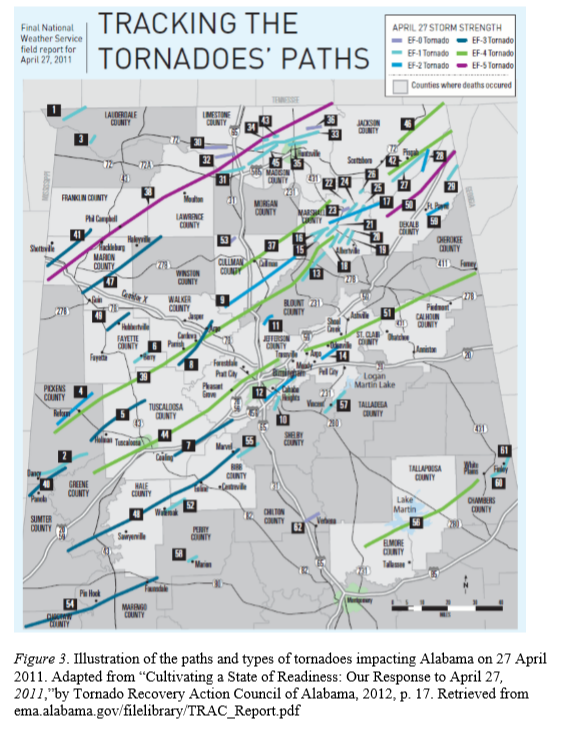
\includegraphics[width=0.4\textwidth]{figures/Tracking_The_Tornadoes_Paths_in_Alabama} 

}

\caption{Example of how exposure to tornadoes was assesses in Christopher (2017) for counties.}\label{fig:unnamed-chunk-3}
\end{figure}

\begin{figure}

{\centering 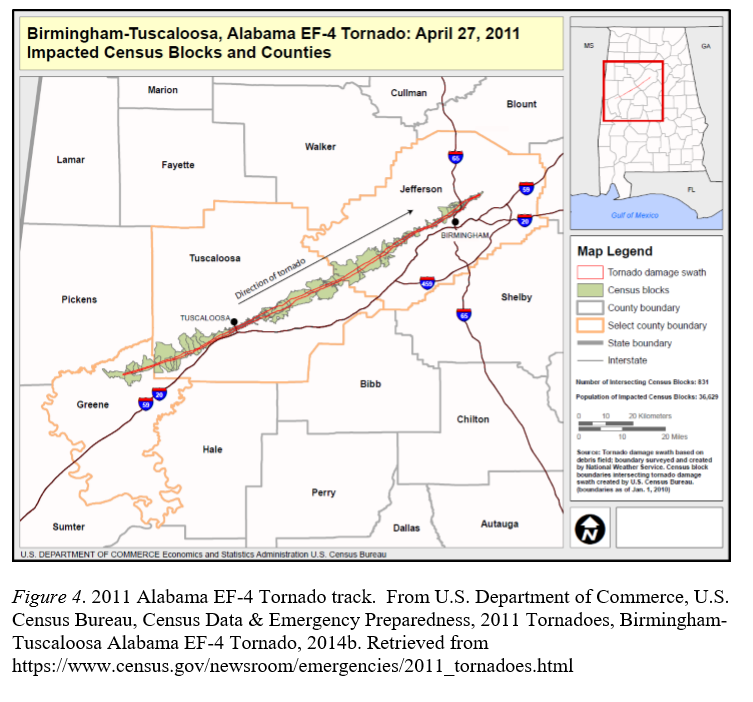
\includegraphics[width=0.4\textwidth]{figures/Birmingham_Tuscaloosa_Tornado_Track} 

}

\caption{Second Figure.}\label{fig:unnamed-chunk-4}
\end{figure}

\hypertarget{zahran2011economics}{%
\section{(Zahran et al. 2011)}\label{zahran2011economics}}

This study investigated mental health outcomes following Hurricanes
Katrina and Rita.

\hypertarget{temporal-scale-17}{%
\subsection{Temporal Scale}\label{temporal-scale-17}}

\begin{itemize}
\tightlist
\item
  ``Mental health condition is measured as the reported count of poor
  mental health days experienced by a respondent in the previous 30
  days. Data on mental health days are from the CDC's BRFSS,
  2005--2006.'' (Zahran et al. 2011)
\item
  {[}They focus only on Hurricanes Katrina and Rita, right?{]}
\item
  {[}Do they have the exact date that the respondent took the survey?
  I'm guessing they just do these surveys once a year or something, in
  which case, they'd have a single outcome measurement for the year or
  the storm, and that wouldn't necessarily be close in time to the
  storm. Is that right? In that case, just a measure at the yearly
  scale, or a cumulative storm measurement, would probably be resolved
  enough temporally for the study.{]}
\end{itemize}

\hypertarget{spatial-scale-17}{%
\subsection{Spatial Scale}\label{spatial-scale-17}}

\begin{itemize}
\tightlist
\item
  Intensity of hurricane's path measured using data on property damage
  and crop loss from the Spatial Hazard Losses and Events Database.
\item
  {[}As a note, I think maybe we mean ``intensity of the hurricane along
  its path'' rather than ``intensity of hurricane's path''{]}
\item
  {[}For the Spatial Hazard Losses and Events Database, could you add
  some details on that? Is that a database these authors created, or is
  it something publicly available? You could check the reference they
  use for this database.{]}
\item
  {[}Based on a comment later, the spatial scale was at the county
  level. It looks like this is the finest resolution they have for each
  respondent, so you wouldn't need more resolved exposure measuments in
  this case.{]}
\item
  {[}Did they use a continuous metric for exposure, or just separate
  into exposed / unexposed based on these damage / losses values in the
  database?{]}
\end{itemize}

\hypertarget{exposure-16}{%
\subsection{Exposure}\label{exposure-16}}

\begin{itemize}
\tightlist
\item
  ``Individual exposure to Hurricane Katrina and/or Rita was determined
  by information on the temporal and spatial coordinates of each
  hurricane event, the date a respondent was interviewed by the CDC, and
  the respondent's place of county residence, as reported in the CDC's
  Behavioral Risk Factor Surveillance System (BRFSS) database'' (Zahran
  et al. 2011)
\item
  {[}Could you clarify for this exposure assessment? Based on one of the
  previous comments, they used damages data, but this is sounding like
  they used how close a county was to the track. Maybe they first used
  distance to the storm to determine exposed / unexposed and then used
  damages data to further distinguish how hard-hit each county was or
  something?{]}
\item
  Number of poor mental healthd days expected to have spikes
  corresponding to hurricane events in affected but not unaffected areas
  with respect to hurricane exposure.
\item
  {[}To clarify, did they use the same time period, but compare by
  location to compare exposed to unexposed? (so, in other words, instead
  of comparing one county over time they compared across counties?). If
  so, I think we definitely want to try to pull some more details on how
  they determined a county was exposed to the storm.{]}
\end{itemize}

\hypertarget{resultsoutcomes-12}{%
\subsection{Results/Outcomes}\label{resultsoutcomes-12}}

\begin{itemize}
\tightlist
\item
  Outcome of interest was mental health resilience of Hurricane Katrina
  and Rita survivors, stratified by vulnerability status. Number of poor
  mental health days used as metric for this.
\item
  Vulnerability status measured by poor physical health, social support,
  education level, income, and being a single mother.
\item
  Single mothers were identified as a particular vulnerability category
  of interest
\item
  ``Resistance refers to the capacity to limit displacement from
  equilibrium following a traumatic event. Resilience, by contrast,
  points to the ability to return to an equilibrium state---the more
  rapid the return to preevent functioning, the greater the
  resilience.'' (Zahran et al. 2011)
\item
  Average number of poor mental health days in 30 was 3.37 for the
  population as a whole, and 5.95 for single mothers.
\item
  Overall, hurricane exposed single mothers and exposed ``others'' all
  experienced an increased number of days of poor mental health.
\item
  ``We estimate that single mothers, as a group, suffered over \$130
  million in productivity loss from added postdisaster stress and
  disability.'' (Zahran et al. 2011)
\end{itemize}

\hypertarget{zahran2013daily}{%
\section{(Zahran, Tavani, and Weiler 2013)}\label{zahran2013daily}}

This study investigates \ldots{}

\hypertarget{temporal-scale-18}{%
\subsection{Temporal Scale}\label{temporal-scale-18}}

\begin{itemize}
\tightlist
\item
  {[}Are these recorded by date, or is there an event-wide estimate of
  total casualties that's used? Do they have a date for each disaster,
  or just the month or year?{]}
\end{itemize}

\hypertarget{spatial-scale-18}{%
\subsection{Spatial Scale}\label{spatial-scale-18}}

\begin{itemize}
\tightlist
\item
  Casualty counts are recorded at the county level in counties affected
  by either hurricanes or tornados.
\item
  {[}So it sounds like this study has outcome data aggregated at the
  county level for the spatial level.{]}
\end{itemize}

\hypertarget{exposure-17}{%
\subsection{Exposure}\label{exposure-17}}

\begin{itemize}
\tightlist
\item
  ``In the event of a natural disaster,people living in affected areas
  suffer both income and wealth losses. Wealth losses typically involve
  damage to residential or commercial property, whereas income losses
  involve lost wages, profits, dividends, and rents in consequence of
  the disaster.'' (Zahran, Tavani, and Weiler 2013)
\item
  {[}It looks like they are looking at the level of county. How have
  they decided if a county is exposed to a hurricane? Are they using a
  disaster database that lists each disaster event for each county? Or
  did they pair up with hurricane tracks or something?{]}
\end{itemize}

\hypertarget{resultsoutcomes-13}{%
\subsection{Results/Outcomes}\label{resultsoutcomes-13}}

\begin{itemize}
\tightlist
\item
  Dependent variables analyzed are hurricane casualties and tornado
  casualties.
\item
  {[}Are these only the casualties that were specifically linked to the
  disaster, or does it measure the total increase in excess deaths
  during the period of the disaster?{]}
\item
  Predictor variables are disaster damage, recency bias, and day of the
  week.
\item
  {[}Could you clarify what ``recency bias'' measures?{]}
\item
  {[}Where are they getting the disaster damage estimates?{]}
\end{itemize}

\hypertarget{nordhaus2010economics}{%
\section{(Nordhaus 2010)}\label{nordhaus2010economics}}

This study investigates patterns in exposure to and damages from
tropical cyclones in the US {[}have I summarized this study
correctly?{]}.

\hypertarget{temporal-scale-19}{%
\subsection{Temporal Scale}\label{temporal-scale-19}}

\begin{itemize}
\tightlist
\item
  Annual number of tropical cyclones from 1970 to 2004 averaged at 85.
\item
  Reliable data on the number of tropical cyclones has only been
  collected since 1960, so it is hard to accurately gage if the average
  number of tropical cyclones per year is increasing.
\item
  ``Using ``best track'' or HURDAT data for North Atlantic storms, there
  has been a clear increase in the frequency of storms over the
  1851--2005 period, particularly since 1980.''
\item
  {[}Are they just using total counts of storms per year? Or are they
  looking at specific storms? This would help us figure out the time
  resolution, and whether it would make sense as yearly or cumulative
  for the storm.{]}
\end{itemize}

\hypertarget{spatial-scale-19}{%
\subsection{Spatial Scale}\label{spatial-scale-19}}

\begin{itemize}
\tightlist
\item
  Study focues on tropical cyclones in the North Atlantic, focusing on
  the East Coast of the United States
\item
  {[}Do they measure patterns by county or state? Or are they really
  pooling everything together to just have one measure across the whole
  east coast?{]}
\end{itemize}

\hypertarget{exposure-18}{%
\subsection{Exposure}\label{exposure-18}}

\begin{itemize}
\tightlist
\item
  Storm intensity is measured by something called ``Hurricane Power''
  which is defined as a function of maximum wind speed squared or cubed
  {[}This is measured separately for each storm, right?{]}
\item
  ``NOAA has constructed a power index called the accumulated cyclone
  energy (ACE) index, which is a function of maximum wind speed
  squared.'' {[}nordhaus2010economics{]}
\item
  This study analyzes economics impacts by looking at three primary
  factors: number of storms, maximum wind speed at landfall, and GDP.
\item
  {[}Is this number of storms per year? How do they aggregate the
  maximum wind speeds across storms, if they're using both the number of
  storms and the maximum wind speed?{]}
\end{itemize}

\hypertarget{resultsoutcomes-14}{%
\subsection{Results/Outcomes}\label{resultsoutcomes-14}}

\begin{itemize}
\tightlist
\item
  Southern Atlantic coast is most vulnerable to hurricanes in the
  context of climate echange
\item
  Damages appear to increase to the ninth degree of wind speed.
\item
  {[}Where do they get their data on economic impacts / damages? Are
  they calculating this themselves or getting it from a database that's
  already been created? If they're calculating it themselves, what are
  the inputs?{]}
\item
  It is estimated that climate change will increase the intensity of
  hurricanes and tropical cyclones, but it isn't clear if it will also
  increase the frequency.
\item
  Based on 2005 incomes, it is estimated that average annual US
  hurricane damages will increase by \$10 billion.
\end{itemize}

\hypertarget{gaddis2007full}{%
\section{(Gaddis et al. 2007)}\label{gaddis2007full}}

\hypertarget{temporal-scale-20}{%
\subsection{Temporal Scale}\label{temporal-scale-20}}

\begin{itemize}
\tightlist
\item
  Built capital recovery is typically measured in the short term because
  it is limited by available human labor and construction materials,
  whereas natural capital recovery may take much longer because it is
  often limited by natural processes.
\item
  Standard discount rate may be appropriate for built capital stocks but
  it is inappropriate to apply it to social, human, and natural capital
  stocks.
\item
  {[}For this study, do they have damages / economic data that they're
  using? If so, what is the time scale? For example, do they have one
  measurement per storm, or maybe are they using data that's collected
  every year?{]}
\end{itemize}

\hypertarget{spatial-scale-20}{%
\subsection{Spatial Scale}\label{spatial-scale-20}}

\begin{itemize}
\tightlist
\item
  Full cost accounting of damages after hurricanes must look at
  regional, national and international scales since communities and
  areas not affected by the direct results of the tropical cyclone or
  hurricane may still be impacted economically.
\item
  It was noted that some regions benefit economically from storms, for
  example areas surrounding New Orleans saw their property values go up
  because of people trying to leave the New Orleans area.
\item
  {[}If this is a quantitative scale (rather than a commentary or
  something), do they have data on damages that they're looking at? In
  that case, do they have those numbers by state or by county or by some
  other aggregation? This is what we'd want to list for the spatial
  scale here.{]}
\end{itemize}

\hypertarget{exposure-19}{%
\subsection{Exposure}\label{exposure-19}}

\begin{itemize}
\tightlist
\item
  Economic damage in the form of built capital, human capital, natural
  capital, and social capital. {[}How do they get these values? Do they
  have a database of damages specifically from tropical cyclones? Or are
  they pairing up economic data from some other source with tropical
  cyclone dates and places?{]}
\end{itemize}

\hypertarget{resultsoutcomes-15}{%
\subsection{Results/Outcomes}\label{resultsoutcomes-15}}

\begin{itemize}
\item
  Current policies that incentivize settling in vulnerable coastal areas
  should be replaced with policies that encourage populating the
  interior of the country which is experiencing negative population
  growth.
\item
\end{itemize}

\hypertarget{narita2009damage}{%
\section{(Narita, Tol, and Anthoff 2009)}\label{narita2009damage}}

\hypertarget{temporal-scale-21}{%
\subsection{Temporal Scale}\label{temporal-scale-21}}

\begin{itemize}
\tightlist
\item
  Model runs from the years 1950 (1950 to 2000 used for model
  calibration) to 3000
\item
  {[}For this study, I think we're also interested in figuring out what
  data they used to make the model that they ultimately use for future
  damages. To project out, they must have some estimate of the
  relationship between damage and tropical cyclones today, and then
  they're using that estimated relationship to project damages in the
  future. In that case, how did they build their model of the
  relationship between tropical cyclones and damages? Did they use
  observed data from previous years? If so, did they have damage
  estimates by storm, or by year, or at some other time scale? We'll
  want to know that to answer the ``temporal'' scale question for this
  paper (and similarly the spatial scale to answer the ``spatial''
  question---in other words, if they had data from the past that they
  used to estimate this association, was it by country or by state or by
  county or at some other aggregation?{]}
\end{itemize}

\hypertarget{spatial-scale-21}{%
\subsection{Spatial Scale}\label{spatial-scale-21}}

\begin{itemize}
\tightlist
\item
  Globe divided into 16 regions to test scenarios.
\item
  {[}Are these regions the level that the data was collected and used to
  build the present-day damages model, though?{]}
\end{itemize}

\hypertarget{exposure-20}{%
\subsection{Exposure}\label{exposure-20}}

\begin{itemize}
\tightlist
\item
  FUND version 3.4 used to analyze climate change impacts attributable
  to enhancement of tropical cyclone activity
\item
  ``Essentially, FUND is a model that calculates damage caused by
  climate change for 16 regions of the world listed in Table 1 by making
  use of exogenous scenarios of socioeconomic variables. The scenarios
  comprise projected temporal profiles of population growth, economic
  growth, autonomous energy efficiency improvements and carbon
  efficiency improvements (decarbonization), emissions of carbon dioxide
  from land use change, and emissions of methane and of nitrous oxide.
  Carbon dioxide emissions from fossil fuel combustion are computed
  endogenously on the basis of the Kaya identity. The calculated impacts
  of climate change perturb the default paths of population and economic
  outputs corresponding to the exogenous scenarios. The model runs from
  the years 1950 to 3000 in time steps of a year, though the outputs for
  the 1950 to 2000 period is only used for calibration, and the years
  beyond 2100 are used for approximating the social cost of carbon under
  low discount rates, a matter that does not concern us in this
  paper.''(Narita, Tol, and Anthoff 2009)
\end{itemize}

\hypertarget{resultsoutcomes-16}{%
\subsection{Results/Outcomes}\label{resultsoutcomes-16}}

\begin{itemize}
\tightlist
\item
  Direct economic damages to the USA calculated to almost USD \$19
  billion.
\end{itemize}

\hypertarget{pistrika2010damage}{%
\section{(Pistrika and Jonkman 2010)}\label{pistrika2010damage}}

\hypertarget{temporal-scale-22}{%
\subsection{Temporal Scale}\label{temporal-scale-22}}

\begin{itemize}
\item
\end{itemize}

\hypertarget{spatial-scale-22}{%
\subsection{Spatial Scale}\label{spatial-scale-22}}

\begin{itemize}
\tightlist
\item
  Greater New Orleans metropolitan area was studied. The area was
  divided into three sections based on ``bowls'' aka polders.
\item
  {[}Can we find out a little bit more about what these ``bowls'' are? I
  assume that they have some geographic definition? This is really
  interesting---it looks like we have a new spatial scale that's
  different from county or ZIP code and is based more on something
  that's meaningful for flooding.{]}
\item
  {[}How do these bowls compare to neighborhoods? Would you have several
  neighborhoods in one, or are they smaller than a neighborhood?{]}
\end{itemize}

\hypertarget{exposure-21}{%
\subsection{Exposure}\label{exposure-21}}

\begin{itemize}
\item
  Hydrodynamic flood simulations used to analyze relationship between
  flood characteristics and damage to buildings.
\item
  {[}In other words, it sounds like they had some model of flooding that
  they could use to simulate floods, and then did they compare those
  outputs to the actual data that was observed after a specific storm to
  buildings? Or is this study purely a simulation study? If it's only a
  simulation study, we probably won't include it, because our focus is
  more on helping to connect observations from a storm with human
  impacts studies, and if it was just a simulation study, it wouldn't
  need observations as inputs, I don't think.{]}
\item
  Momentum = mass x velocity = density x volume x velocity
  =\textgreater{} Momentum = density x flooded horizontal area x (depth
  x velocity)
\item
  Characteristics of the flood (load/flood action) and building
  resistance and are used to predict the structural damage. This then is
  used to analyze and predict the economic damage by looking at the
  total replacement cost and the building's market cost prior to the
  disaster.
\end{itemize}

\hypertarget{resultsoutcome-3}{%
\subsection{Results/Outcome}\label{resultsoutcome-3}}

\begin{itemize}
\tightlist
\item
  Outcome of interest is direct damage to residential buildings in New
  Orleans caused by flooding after Hurricane Katrina {[}Hmmm. Again, it
  would be helpful to clarify here if they were using real data on the
  damage observed to buildings after that storm?{]}
\item
  ``The spatial level of detail of the analysis is a determining factor
  for the correlation between predictions and observations. The smaller
  the spatial unit of the analysis the poorer the relationship between
  flood characteristics and damage.'' (Pistrika and Jonkman 2010)
\item
  ``The highest damage percentages and structural damage mainly occurred
  in areas where higher flow velocities occurred, especially near the
  breaches in the Lower 9th Ward neighborhood. Due to the approach that
  was used for damage quantification, buildings that sustained
  structural damage, had damage levels higher than 50\% of their market
  value.'' (Pistrika and Jonkman 2010)
\item
  ``An alternative approach has been proposed that could be used to
  distinguish three different damage zones based on the combination of
  water depth and flow velocity. There appeared to be clear differences
  between the average, observed damage values in the three zones. This
  approach could be useful to determine the extent of flood damage and
  distinguish the main damage zones for an area affected by flooding due
  to breaching of flood defenses.'' (Pistrika and Jonkman 2010)
\item
  {[}Again, can you tell if they were using \emph{observations} about
  the water depth and flow velocity during Hurricane Katrina for this
  analysis, or did they just simulate what they expected those to be,
  based on some flood simulation model, rather than use real
  observations? If they used real observations, then I think we need to
  find out a bit more about how they got those. Did they put out their
  own sensors to collect it? Or were they using data from the USGS, for
  example?{]}
\end{itemize}

\hypertarget{xian2015storm}{%
\section{(Xian, Lin, and Hatzikyriakou 2015)}\label{xian2015storm}}

FEMA's flood risk mapping techniques are tested against a survey
quantitatively assessing the damage to 380 structures in Ortley Beach,
New Jersey, after Hurricane Sandy in 2012.

\hypertarget{temporal-scale-23}{%
\subsection{Temporal Scale}\label{temporal-scale-23}}

\begin{itemize}
\tightlist
\item
  Damage was surveyed in the aftermath of Hurricane Sandy
\end{itemize}

\hypertarget{spatial-scale-23}{%
\subsection{Spatial Scale}\label{spatial-scale-23}}

\begin{itemize}
\tightlist
\item
  380 structures in a heavily affected area of Ortley Beach
\end{itemize}

\hypertarget{exposure-22}{%
\subsection{Exposure}\label{exposure-22}}

\begin{itemize}
\tightlist
\item
  ``we quantitatively measure the damage percentage for each of the
  significant building components (foundation, exterior walls, wall
  siding, windows, doors, roof, and roof cover). Moreover, we assess the
  damage percentage to each component at each story and each side of a
  structure. The survey indicates that different sides and stories of a
  structure suffered different levels of damage due to the different
  surge/wave effects.'' (Xian, Lin, and Hatzikyriakou 2015)
\item
  Different factors were put in a database: Distance from the coast,
  ground elevation, elevation above ground, and year building was built.
\end{itemize}

\hypertarget{resultsoutcome-4}{%
\subsection{Results/Outcome}\label{resultsoutcome-4}}

\begin{itemize}
\tightlist
\item
  Overall, the side facing the ocean, and the first floor of a building
  were typically at a greater risk for damage than the other three sides
  and other floors.
\item
  Buildings built after 1979 tended to withstand damage from the
  hurricanes greater than buildings built before this year.
\end{itemize}

\hypertarget{willison2019quantifying}{%
\section{(Willison et al. 2019)}\label{willison2019quantifying}}

Quantifying the US federal response and resulting inequality in Texas
and Florida versus Puerto Rico. Hurricanes Irma, Harvey, and Maria are
all analyzed.

\hypertarget{temporal-scale-24}{%
\subsection{Temporal Scale}\label{temporal-scale-24}}

\begin{itemize}
\tightlist
\item
  Analysis spans landfall to six months after each hurricane, in this
  case Harvey, Irma, and Maria.
\end{itemize}

\hypertarget{spatial-scale-24}{%
\subsection{Spatial Scale}\label{spatial-scale-24}}

\begin{itemize}
\tightlist
\item
  Florida, Texas, and Puerto Rico were all analyzed at the
  state/territory level.
\end{itemize}

\hypertarget{exposure-23}{%
\subsection{Exposure}\label{exposure-23}}

\begin{itemize}
\tightlist
\item
  ``To examine differences in disaster responses across the three
  hurricanes, we focus on measures of federal spending, federal
  resources distributed and direct and indirect storm-mortality counts.
  Federal spending estimates come from congressional appropriations and
  FEMA records. Resource estimates come from FEMA documents and news
  releases. Mortality counts come from National Oceanographic and
  Atmospheric Administration (NOAA) reports, respective vital statistics
  offices and news reports. Damage estimates came from NOAA reports. In
  each case, we compare the responses and the severity at critical time
  points after the storm.'' (Willison et al. 2019)
\end{itemize}

\hypertarget{resultsoutcome-5}{%
\subsection{Results/Outcome}\label{resultsoutcome-5}}

\begin{itemize}
\tightlist
\item
  ``Our results show that the federal response was faster and more
  generous across measures of money and staffing to Hurricanes Harvey
  and Irma in Texas and Florida, compared with Hurricane Maria in Puerto
  Rico. This result would be unsurprising if Hurricane Maria was less
  damaging than Irma and Harvey. However, Hurricanes Harvey and Irma
  made landfall as category four hurricanes,1 5 and Maria hit Puerto
  Rico as a `high-end' category 4, or just below the threshold of a
  category 5 hurricane.6 Maria caused more damage in Puerto Rico than
  Irma in Florida or Harvey in Texas in terms of loss of electricity and
  housing destruction,1 5 6 with overall damage estimates comparable to
  Harvey, and greater than estimates for Irma.1 Assuming that
  infrastructure costs are higher in Texas and Florida, and therefore
  more expensive to repair, compared with Puerto Rico, the high damage
  estimates in Puerto Rico emphasise the severity of storm damage.''
  (Willison et al. 2019)
\end{itemize}

\hypertarget{xian2018brief}{%
\section{(Xian et al. 2018)}\label{xian2018brief}}

Hydrodynamic storm surge and wave modeling was coupled with rapid damage
surveying in the Florida Keys to assess physical damage.

\hypertarget{temporal-scale-25}{%
\subsection{Temporal Scale}\label{temporal-scale-25}}

\begin{itemize}
\tightlist
\item
  Field surveys were carried out September 21-24 soon after Hurricane
  Irma (September 10 is when it made landfall).
\item
  Rapid survey method involved driving at a speed of 10 mph throughout
  affected areas and taking GPS informed pictures from the rear side
  windows.
\end{itemize}

\hypertarget{spatial-scale-25}{%
\subsection{Spatial Scale}\label{spatial-scale-25}}

\begin{itemize}
\tightlist
\item
  Big Pine Key and Marathon are the two survey locations in the Florida
  Keys, they were the two areas that were most affected by the
  hurricane.
\item
  Over 1600 residential buildings were surveyed using the rapid survey
  method.
\end{itemize}

\hypertarget{exposure-24}{%
\subsection{Exposure}\label{exposure-24}}

\begin{itemize}
\tightlist
\item
  After conducting a damage and assessment survey after Hurricane Irma,
  a statistical regression approach is used to quantify the contribution
  of various hazard and vulnerability factors.
\item
  ``To understand the hazard and inform the field survey, we first use
  the coupled hydrodynamic and 41 wave model ADCIRC+SWAN (Dietrich et
  al.~2012, Marsooli and Lin 2017) to simulate the 42 storm tide (i.e.,
  water level) and wave height for Hurricane Irma. To simulate Irma's
  storm tide 43 and wave (Figure 1), we apply the surface wind (at 10-m)
  and sea-level pressure fields from 44 National Center for
  Environmental Prediction Final (NCEP FNL) operational global analysis
  data (0.25o x 0.25o 45 x 6 hours).'' (Xian et al. 2018)
\item
  The collected photos and satellite images are used to categorize
  damage state for each residential building surveyed.
\item
  FEMA's damage state criteria that were used in Hurricane Sandy are
  used to categorize and assess the damage in Big Pine Key and Marathon,
  and include the categories No/very limited damage; Minor damage; Minor
  damage; and Destroyed.
\end{itemize}

\hypertarget{resultsoutcome-6}{%
\subsection{Results/Outcome}\label{resultsoutcome-6}}

\begin{itemize}
\tightlist
\item
  Hydrodynamic forces induced by storm surges and waves were the primary
  cause of destroyed and heaviliy damaged buildings.
\item
  Observed storm surge damage is consistent with the hydrodynamic
  models.
\item
  Analysis on Big Pine Key revealed that distance from the coastline was
  the most significant predictor for damage state
\item
  On Marathon, building type and size were the two main predictors.
\end{itemize}

\hypertarget{shao2017understanding}{%
\section{(Shao et al. 2017)}\label{shao2017understanding}}

This study focuses on the effects of external influences and perceptions
of flood risk on individual's behavior relating to purchasing flooding
insurance. Flood insurance ownership rates are relatively low and
despite the fact that home owners in Special Flood Hazard Areas are
required to buy flood insurance if they are receiving a mortgage from a
federally backed or regulated lender, the law is not heavily enforced.

\hypertarget{temporal-scale-26}{%
\subsection{Temporal Scale}\label{temporal-scale-26}}

\begin{itemize}
\tightlist
\item
  Individual levels variables constructed from data collected in 2012
  Gulf Coast Climate Change Study
\item
  Data collected by phone interviews from January 3rd through April 4,
  2012.
\end{itemize}

\hypertarget{spatial-scale-26}{%
\subsection{Spatial Scale}\label{spatial-scale-26}}

\begin{itemize}
\tightlist
\item
  State level
\item
  Stratified random sampling strategy drew independent samples in Texas,
  Louisiana, Mississippi, Alabama, and Florida.
\item
  Contextual variables pertaining to flooding risk taken at the county
  level in these states.
\end{itemize}

\hypertarget{exposure-25}{%
\subsection{Exposure}\label{exposure-25}}

\begin{itemize}
\tightlist
\item
  3856 respondants, response rate was 17.6\%
\end{itemize}

\hypertarget{dependent-variables}{%
\subsubsection{Dependent Variables}\label{dependent-variables}}

\begin{itemize}
\tightlist
\item
  ``The two dependent variables are based on responses to two survey
  questions. The two questions are `do you haveflood insurance?' and `do
  you have flood insurance to feel safer or because it is required?'\,''
  (Shao et al. 2017)
\end{itemize}

\hypertarget{independent-variables}{%
\subsubsection{Independent Variables}\label{independent-variables}}

\begin{itemize}
\tightlist
\item
  ``The individual-level independent variables, including
  socio-demographic features, home ownership, distance from the
  coast(self-reported), trust in the local government and flood-related
  risk perceptions, are all constructed based on survey items.'' (Shao
  et al. 2017)
\item
  ``The contextual variables include spatial information about flood
  hazards estimated by FEMA, peak height of storm surge from the most
  recent hurricane landfall, and economic damages from the most recent
  and most impacted flooding events, respectively. They are all at
  county-level''
\end{itemize}

\hypertarget{resultsoutcome-7}{%
\subsection{Results/Outcome}\label{resultsoutcome-7}}

\begin{itemize}
\tightlist
\item
  People from racial minorities were more likely to buy flood insurance
  voluntarily than whites when controlling for other variables, perhaps
  reflecting that whites perceive less risk than minorities.
\item
  People of higher socioeconomic status (both higher levels of education
  and income) were more likely to buy flood insurance.
\item
  A perception that flooding and storm intensity is increasing also made
  coastal residents more likely to buy flood insurance.
\item
  The other major factors in predicting whether or not a resident would
  buy flood insurance were self reported distance from the coast, and
  belief in local government's preparedness to address climate change.
\end{itemize}

\hypertarget{xian2017optimal}{%
\section{(Xian, Lin, and Kunreuther 2017)}\label{xian2017optimal}}

This paper is about creating an economically optimal elevation level
(OEL), because it is more economical to use this rather than 1 foot
above base flood elevation (BSE). ``Under the regulations of both ASCE
242 and NFIP, FEMA requires coastal houses with repetitive losses and/or
substantial damage from flood events to be elevated to at least 1 foot
above the BFE and recommends all houses in SFHA to be elevated to this
level (FEMA, 2011). However,this requirement/recommendation does not
provide guidance for home owners about how many feet exactly their
houses should be raised to.''(Xian, Lin, and Kunreuther 2017)

\hypertarget{temporal-scale-27}{%
\subsection{Temporal Scale}\label{temporal-scale-27}}

\begin{itemize}
\tightlist
\item
  ``The house information data used in this study, including location,
  ground elevation, house size, and house value, were collected by a
  team of students and faculty from University of Notre Dame and
  Princeton University in an onsite survey three weeks after Sandy.''
  (Xian, Lin, and Kunreuther 2017)
\end{itemize}

\hypertarget{spatial-scale-27}{%
\subsection{Spatial Scale}\label{spatial-scale-27}}

\begin{itemize}
\tightlist
\item
  Three actual houses in Ortley Beach, New Jersey were used to test the
  OEL model.
\end{itemize}

\hypertarget{exposure-26}{%
\subsection{Exposure}\label{exposure-26}}

\begin{itemize}
\tightlist
\item
  ``We propose that an economically optimal elevation level (OEL)for
  coastal houses can be estimated through a cost-benefit analysis(CBA).
  Specifically, the OEL can be calculated as the level that minimizes
  the sum of the upfront elevation cost and present value of cumulative
  annual expected losses over the lifespan of a house.''(Xian, Lin, and
  Kunreuther 2017)
\end{itemize}

\hypertarget{resultsoutcome-8}{%
\subsection{Results/Outcome}\label{resultsoutcome-8}}

\begin{itemize}
\tightlist
\item
  About half of the houses at Ortley Beach would save 10,000 dollars per
  structure if elevated to OELs instead of 1-foot freeboard, and about
  5\% of the houses could save up to 100,000 dollars.
\end{itemize}

\hypertarget{deryugina2018economic}{%
\section{(Deryugina, Kawano, and Levitt
2018)}\label{deryugina2018economic}}

\hypertarget{temporal-scale-28}{%
\subsection{Temporal Scale}\label{temporal-scale-28}}

\begin{itemize}
\tightlist
\item
  Data taken from individual Federal tax returns and third party
  information returns filed between 1999 and 2013.
\end{itemize}

\hypertarget{spatial-scale-28}{%
\subsection{Spatial Scale}\label{spatial-scale-28}}

\begin{itemize}
\tightlist
\item
  City of New Orleans, Louisiana is the focus of the study and New
  Orleans residents were identified as those with a New Orleans zip code
  on their tax return or on their W2 form.
\item
  Cities with similar characteristics to Louisiana are compared, with
  three pre-Katrina dimensions: median earnings, population growth rate,
  and percentage of the population that is black. These cities were
  Baltimore, MD, Birmingham, AL, Detroit, MI, Gary, IN, Jackson, MS,
  Memphis, TN, Newark, NJ, Portsmouth, VA, Richmond, VA, and St.~Louis,
  MO.
\end{itemize}

\hypertarget{exposure-27}{%
\subsection{Exposure}\label{exposure-27}}

\begin{itemize}
\tightlist
\item
  ``We explore five key dimensions across which one might expect the
  economic impact of the hurricane to be heterogeneous: whether a
  household's own home was severely affected by the storm, pre-Katrina
  income, age, homeownership, and whether the household left New
  Orleans.'' (Deryugina, Kawano, and Levitt 2018)
\end{itemize}

\hypertarget{resultsoutcomes-17}{%
\subsection{Results/Outcomes}\label{resultsoutcomes-17}}

\begin{itemize}
\tightlist
\item
  After a few years, the income of New Orleans residents affected by
  Hurricane Katrina actually recovered and surpassed that of controls in
  other cities.
\end{itemize}

\hypertarget{shao2017understanding-1}{%
\section{(Shao et al. 2017)}\label{shao2017understanding-1}}

This is a different article than the other one with the name
shao2017understanding. This one is about perception of increasing
hurricane strengths in the Gulf States.

\hypertarget{temporal-scale-29}{%
\subsection{Temporal Scale}\label{temporal-scale-29}}

\begin{itemize}
\tightlist
\item
  Individual levels variables constructed from data collected in 2012
  Gulf Coast Climate Change Study
\item
  Data collected by phone interviews from January 3rd through April 4,
  2012.
\item
  Previous hurricanes that made landfall were used from the past 20 year
  period of 1992 to 2011.
\end{itemize}

\hypertarget{spatial-scale-29}{%
\subsection{Spatial Scale}\label{spatial-scale-29}}

\begin{itemize}
\tightlist
\item
  State level
\item
  Stratified random sampling strategy drew independent samples in Texas,
  Louisiana, Mississippi, Alabama, and Florida.
\item
  Respondants had to have lived in coastal counties with at least one
  hurricane landfall between 1992 and 2011. (The reasoning is that
  hurricanes don't often occur at a single location, and human memory is
  short so anything past 20 years wouldn't be accurate).
\end{itemize}

\hypertarget{exposure-28}{%
\subsection{Exposure}\label{exposure-28}}

\begin{itemize}
\tightlist
\item
  Spatial pattern of perception of increasing hurricane strength is
  mapped and used as the dependent variable.
\item
  Hurricane strength is measured by maximum windspeed at landfall, storm
  surge, and economic damage.
\end{itemize}

\hypertarget{resultsoutcomes-18}{%
\subsection{Results/Outcomes}\label{resultsoutcomes-18}}

\begin{itemize}
\tightlist
\item
  Outcome of interest is coastal residents' perceptions of increased
  hurricane strength. Intensity of past hurricanes, physical
  characteristics like wind speed, consequences such as economic damage,
  and people's opinions of climate change are the four factors that are
  framed as research questions to see how they affect this perception of
  increased hurricane strength.
\item
  Perceptions of increasing hurricane strength are stronger in Louisiana
  and Mississippi, likely because of memory of Hurricane Katrina, and
  less strong moving away from this epicenter into the Gulf Coasts of
  Texas and Florida.
\end{itemize}

(Grech and Scherb 2015)

This study looked at whether or not Hurricane Katrina had an influence
on the male/female ratio of births in the Gulf states.

\hypertarget{temporal-scale-30}{%
\subsection{Temporal Scale}\label{temporal-scale-30}}

\begin{itemize}
\tightlist
\item
  January 2003 to December 2012 was the time frame from which live birth
  data was collected and analyzed.
\item
  Precipitation data was collected from the US National Weather Service
  and in this study a precipitation map is presented from August 29 to
  September 1, 2005.
\end{itemize}

\hypertarget{spatial-scale-30}{%
\subsection{Spatial Scale}\label{spatial-scale-30}}

\begin{itemize}
\tightlist
\item
  State level
\item
  Data on monthly male and female live births were obtained from the
  CDC's website for the states of Alabama, Florida, Louisiana, and
  Mississippi.
\end{itemize}

\hypertarget{exposure-29}{%
\subsection{Exposure}\label{exposure-29}}

\begin{itemize}
\tightlist
\item
  In this study, precipitation mainly in the form of rainfall was the
  metric for assessing hurricane exposure.
\end{itemize}

\hypertarget{resultsoutcomes-19}{%
\subsection{Results/Outcomes}\label{resultsoutcomes-19}}

\begin{itemize}
\tightlist
\item
  A dose-response relationship was observed between rainfall and the
  male to female sex ratio of live births 8 to 10 months later.
\item
  " 8--10 months (April to June 2006) after the hurricane, M/F jumped
  significantly from 1.052 to 1.071 with a SOR of 1.018 " (Grech and
  Scherb 2015)
\end{itemize}

\hypertarget{references}{%
\section*{References}\label{references}}
\addcontentsline{toc}{section}{References}

\hypertarget{refs}{}
\leavevmode\hypertarget{ref-bayleyegn2006rapid}{}%
Bayleyegn, Tesfaye, Amy Wolkin, Kathleen Oberst, Stacy Young, Carlos
Sanchez, Annette Phelps, Joann Schulte, Carol Rubin, and Dahna Batts.
2006. ``Rapid Assessment of the Needs and Health Status in Santa Rosa
and Escambia Counties, Florida, After Hurricane Ivan, September 2004.''
\emph{Disaster Management \& Response} 4 (1): 12--18.

\leavevmode\hypertarget{ref-bevilacqua2020understanding}{}%
Bevilacqua, Kristin, Rehana Rasul, Samantha Schneider, Maria Guzman,
Vishnu Nepal, Deborah Banerjee, Joann Schulte, and Rebecca M Schwartz.
2020. ``Understanding Associations Between Hurricane Harvey Exposure and
Mental Health Symptoms Among Greater Houston-Area Residents.''
\emph{Disaster Medicine and Public Health Preparedness}, 1--8.

\leavevmode\hypertarget{ref-bianchette2009ecological}{}%
Bianchette, TA, K-B Liu, NS-N Lam, and LM Kiage. 2009. ``Ecological
Impacts of Hurricane Ivan on the Gulf Coast of Alabama: A Remote Sensing
Study.'' \emph{Journal of Coastal Research}, 1622--6.

\leavevmode\hypertarget{ref-bourque2006weathering}{}%
Bourque, Linda B, Judith M Siegel, Megumi Kano, and Michele M Wood.
2006. ``Weathering the Storm: The Impact of Hurricanes on Physical and
Mental Health.'' \emph{The Annals of the American Academy of Political
and Social Science} 604 (1): 129--51.

\leavevmode\hypertarget{ref-christopher2017effects}{}%
Christopher, Kenneth E. 2017. ``The Effects of Hurricane and Tornado
Disasters on Pregnancy Outcomes.'' PhD thesis, Walden University.

\leavevmode\hypertarget{ref-deryugina2018economic}{}%
Deryugina, Tatyana, Laura Kawano, and Steven Levitt. 2018. ``The
Economic Impact of Hurricane Katrina on Its Victims: Evidence from
Individual Tax Returns.'' \emph{American Economic Journal: Applied
Economics} 10 (2): 202--33.

\leavevmode\hypertarget{ref-ferdinand2005hurricane}{}%
Ferdinand, Keith C. 2005. ``The Hurricane Katrina Disaster: Focus on the
Hypertensive Patient.'' \emph{The Journal of Clinical Hypertension} 7
(11): 679--80.

\leavevmode\hypertarget{ref-gaddis2007full}{}%
Gaddis, Erica Brown, Brian Miles, Stephanie Morse, and Debby Lewis.
2007. ``Full-Cost Accounting of Coastal Disasters in the United States:
Implications for Planning and Preparedness.'' \emph{Ecological
Economics} 63 (2-3): 307--18.

\leavevmode\hypertarget{ref-grabich2016measuring}{}%
Grabich, SC, J Horney, C Konrad, and DT Lobdell. 2016. ``Measuring the
Storm: Methods of Quantifying Hurricane Exposure with Pregnancy
Outcomes.'' \emph{Natural Hazards Review} 17 (1): 06015002.

\leavevmode\hypertarget{ref-grabich2016hurricane}{}%
Grabich, Shannon C, Whitney R Robinson, Stephanie M Engel, Charles E
Konrad, David B Richardson, and Jennifer A Horney. 2016. ``Hurricane
Charley Exposure and Hazard of Preterm Delivery, Florida 2004.''
\emph{Maternal and Child Health Journal} 20 (12): 2474--82.

\leavevmode\hypertarget{ref-grech2015hurricane}{}%
Grech, Victor, and Hagen Scherb. 2015. ``Hurricane Katrina: Influence on
the Male-to-Female Birth Ratio.'' \emph{Medical Principles and Practice}
24 (5): 477--85.

\leavevmode\hypertarget{ref-hagy2006effects}{}%
Hagy, James D, John C Lehrter, and Michael C Murrell. 2006. ``Effects of
Hurricane Ivan on Water Quality in Pensacola Bay, Florida.''
\emph{Estuaries and Coasts} 29 (6): 919--25.

\leavevmode\hypertarget{ref-harville2010population}{}%
Harville, Emily W, Tri Tran, Xu Xiong, and Pierre Buekens. 2010.
``Population Changes, Racial/Ethnic Disparities, and Birth Outcomes in
Louisiana After Hurricane Katrina.'' \emph{Disaster Medicine and Public
Health Preparedness} 4 (S1): S39--S45.

\leavevmode\hypertarget{ref-jaycox2010children}{}%
Jaycox, Lisa H, Judith A Cohen, Anthony P Mannarino, Douglas W Walker,
Audra K Langley, Kate L Gegenheimer, Molly Scott, and Matthias Schonlau.
2010. ``Children's Mental Health Care Following Hurricane Katrina: A
Field Trial of Trauma-Focused Psychotherapies.'' \emph{Journal of
Traumatic Stress: Official Publication of the International Society for
Traumatic Stress Studies} 23 (2): 223--31.

\leavevmode\hypertarget{ref-kinney2008autism}{}%
Kinney, Dennis K, Andrea M Miller, David J Crowley, Emerald Huang, and
Erika Gerber. 2008. ``Autism Prevalence Following Prenatal Exposure to
Hurricanes and Tropical Storms in Louisiana.'' \emph{Journal of Autism
and Developmental Disorders} 38 (3): 481--88.

\leavevmode\hypertarget{ref-lane2013health}{}%
Lane, Kathryn, Kizzy Charles-Guzman, Katherine Wheeler, Zaynah Abid,
Nathan Graber, and Thomas Matte. 2013. ``Health Effects of Coastal
Storms and Flooding in Urban Areas: A Review and Vulnerability
Assessment.'' \emph{Journal of Environmental and Public Health} 2013.

\leavevmode\hypertarget{ref-lieberman2017self}{}%
Lieberman-Cribbin, Wil, Bian Liu, Samantha Schneider, Rebecca Schwartz,
and Emanuela Taioli. 2017. ``Self-Reported and Fema Flood Exposure
Assessment After Hurricane Sandy: Association with Mental Health
Outcomes.'' \emph{PLoS One} 12 (1): e0170965.

\leavevmode\hypertarget{ref-narita2009damage}{}%
Narita, Daiju, Richard SJ Tol, and David Anthoff. 2009. ``Damage Costs
of Climate Change Through Intensification of Tropical Cyclone
Activities: An Application of Fund.'' \emph{Climate Research} 39 (2):
87--97.

\leavevmode\hypertarget{ref-nordhaus2010economics}{}%
Nordhaus, William D. 2010. ``The Economics of Hurricanes and
Implications of Global Warming.'' \emph{Climate Change Economics} 1
(01): 1--20.

\leavevmode\hypertarget{ref-pistrika2010damage}{}%
Pistrika, Aimilia K, and Sebastiaan N Jonkman. 2010. ``Damage to
Residential Buildings Due to Flooding of New Orleans After Hurricane
Katrina.'' \emph{Natural Hazards} 54 (2): 413--34.

\leavevmode\hypertarget{ref-pugatch2019tropical}{}%
Pugatch, Todd. 2019. ``Tropical Storms and Mortality Under Climate
Change.'' \emph{World Development} 117: 172--82.

\leavevmode\hypertarget{ref-scaramutti2019mental}{}%
Scaramutti, Carolina, Christopher P Salas-Wright, Saskia R Vos, and Seth
J Schwartz. 2019. ``The Mental Health Impact of Hurricane Maria on
Puerto Ricans in Puerto Rico and Florida.'' \emph{Disaster Medicine and
Public Health Preparedness} 13 (1): 24--27.

\leavevmode\hypertarget{ref-schwartz2018preliminary}{}%
Schwartz, Rebecca M, Stephanie Tuminello, Samantha M Kerath, Janelle
Rios, Wil Lieberman-Cribbin, and Emanuela Taioli. 2018. ``Preliminary
Assessment of Hurricane Harvey Exposures and Mental Health Impact.''
\emph{International Journal of Environmental Research and Public Health}
15 (5): 974.

\leavevmode\hypertarget{ref-shao2017understanding}{}%
Shao, Wanyun, Siyuan Xian, Barry D Keim, Kirby Goidel, and Ning Lin.
2017. ``Understanding Perceptions of Changing Hurricane Strength Along
the Us Gulf Coast.'' \emph{International Journal of Climatology} 37 (4):
1716--27.

\leavevmode\hypertarget{ref-willison2019quantifying}{}%
Willison, Charley E, Phillip M Singer, Melissa S Creary, and Scott L
Greer. 2019. ``Quantifying Inequities in Us Federal Response to
Hurricane Disaster in Texas and Florida Compared with Puerto Rico.''
\emph{BMJ Global Health} 4 (1).

\leavevmode\hypertarget{ref-xian2018brief}{}%
Xian, Siyuan, Kairui Feng, Ning Lin, Reza Marsooli, Daniel Chavas, Jie
Chen, and Adam Hatzikyriakou. 2018. ``Brief Communication: Rapid
Assessment of Damaged Residential Buildings in the Florida Keys After
Hurricane Irma.'' \emph{Natural Hazards and Earth System Sciences} 18
(7).

\leavevmode\hypertarget{ref-xian2015storm}{}%
Xian, Siyuan, Ning Lin, and Adam Hatzikyriakou. 2015. ``Storm Surge
Damage to Residential Areas: A Quantitative Analysis for Hurricane Sandy
in Comparison with Fema Flood Map.'' \emph{Natural Hazards} 79 (3):
1867--88.

\leavevmode\hypertarget{ref-xian2017optimal}{}%
Xian, Siyuan, Ning Lin, and Howard Kunreuther. 2017. ``Optimal House
Elevation for Reducing Flood-Related Losses.'' \emph{Journal of
Hydrology} 548: 63--74.

\leavevmode\hypertarget{ref-zahran2011economics}{}%
Zahran, Sammy, Lori Peek, Jeffrey G Snodgrass, Stephan Weiler, and Lynn
Hempel. 2011. ``Economics of Disaster Risk, Social Vulnerability, and
Mental Health Resilience.'' \emph{Risk Analysis: An International
Journal} 31 (7): 1107--19.

\leavevmode\hypertarget{ref-zahran2013daily}{}%
Zahran, Sammy, Daniele Tavani, and Stephan Weiler. 2013. ``Daily
Variation in Natural Disaster Casualties: Information Flows, Safety, and
Opportunity Costs in Tornado Versus Hurricane Strikes.'' \emph{Risk
Analysis} 33 (7): 1265--80.

\end{document}
